%%%%%%%%%%%%%%%%%%%%%%%%%%%%%%%%%%%%%%%%%%%%%%%%%%%%%%%%%%%%%%%%%%%%%%%%%%%%%%%
% template.tex - version 0.9.1.1 (5/26/2011)
%
% This is a template file for the osudiss-2 class. See
% osudiss-2.pdf for documentation, and the GS material 
% for the requirements.
%
% Copy the following osudiss-2 files your latex path (or just the folder containing this file):
% osudiss-2.cls (v0.9.1)
% sa-draftwater.sty
%
% Then, to compile this file:
% latex template
% bibtex template
% latex template
% latex template
%
% (You can also use pdflatex if you prefer.)
%
%%%%%%%%%%%%%%%%%%%%%%%%%%%%%%%%%%%%%%%%%%%%%%%%%%%%%%%%%%%%%%%%%%%%%%%%%%%%%%%
\documentclass[11pt, onehalf, phd]{osudiss-2} 
% Look at \DeclareOption in osudiss-2.cls for options to change oneside to twoside etc.
% The `11pt' option is unnecessary since it is the default

% `onehalf' sets the line spacing to one-and-a-half spacing instead of
% double spacing.

% The `phd' option is unnecessary since it is the default

% Remove `draft' option for final draft

%%%%%%%%%%%%%%%%%%%%%%%%% Packages %%%%%%%%%%%%%%%%%%%%%%%%%
% Load your favorite packages here
\usepackage{graphicx} % for importing images in figures - you definitely want this!
\usepackage{lipsum} % for fake latin text---you probably don't want this

% For instance... see osudiss-2.pdf for some suggestions, if you don't
% have a clue
\usepackage{bm} % for bold math---useful
\usepackage{booktabs} % for more professional tables

%hyperref packages and options
\usepackage{bookmark} % helps booksmarks look better in PDF
%hypersetup option 'breaklinks' is reguired for line wrapping in the table of contents during latex compilation, and can be removed if you use pdflatex
\hypersetup{colorlinks=true,linkcolor=blue, breaklinks} %internal links in blue, citations in green
%\hypersetup{colorlinks=true,linkcolor=black, citecolor=black, breaklinks} %all links in black
\usepackage[all]{hypcap}

%Use of natbib is STRONGLY recommended to sort and compress your references within each citation
%With these options, natbib will convert i.e. [5,3,9,4] to [3-5, 9]
\usepackage[sort&compress]{natbib}

%required to have latex automatically generate subfigures (i.e. (a), (b) etc)
\usepackage{subfig}

\usepackage{amsmath}
\usepackage{amssymb}
\usepackage{cleveref}
\usepackage{siunitx}

%load glossaries packages
%\usepackage[acronym, section=chapter]{glossaries}
\usepackage[acronym, automake, section=chapter]{glossaries} % recommended if supported by your OS
\makeglossaries %required to actually make a glossary
%A list of common acronyms
%Only those used will be displayed, so you can just add to this list
\newacronym{LLNL}{LLNL}{Lawrence Livermore National Laboratory}
\newacronym{LANL}{LANL}{Los Alamos National Laboratory}
\newacronym{NIF}{NIF}{National Ignition Facility}
\newacronym{NIF-ARC}{NIF-ARC}{National Ignition Facility - Advanced Radiographic Capability}
\newacronym{OMEGA-EP}{OMEGA-EP}{OMEGA Extended Performance System}
\newacronym{RF}{RF}{radio frequency}
\newacronym{QCD}{QCD}{quantum chromodynamics}
\newacronym{QED}{QED}{quantum electrodynamics}
\newacronym{WKB}{WKB}{Wentzel-Kramers-Brillouin}
\newacronym{SRIM}{SRIM}{stopping range of ions in matter}
\newacronym{SOBP}{SOBP}{spread-out Bragg peak}
\newacronym{OSUCCC}{OSUCCC}{The Ohio State Comprehensive Cancer Center}
\newacronym{LLE}{LLE}{Laboratory for Laser Energetics}
\newacronym{TNSA}{TNSA}{target normal sheath acceleration}
\newacronym{IBA}{IBA}{Ion Beam Analysis}
\newacronym{IMPT}{IMPT}{intensity modulated proton therapy}
\newacronym{ALLS}{ALLS}{Advanced Laser Light Source}
\newacronym{XPIF}{XPIF}{x-ray and particle-induced fluorescence}
\newacronym{EDX}{EDX}{energy dispersive x-ray fluorescence}
\newacronym{TEM}{TEM}{transverse electromagnetic mode}
\newacronym{FWHM}{FWHM}{full width at half maximum}
\newacronym{eTNSA}{eTNSA}{enhanced target normal sheath acceleration}
\newacronym{LWFA}{LWFA}{laser wakefield acceleration}
\newacronym{PIC}{PIC}{particle-in-cell}
\newacronym{NGP}{NGP}{nearest grid point}
\newacronym{CCD}{CCD}{charge coupled device}
\newacronym{RPA}{RPA}{radiation pressure acceleration}
\newacronym{LSP}{LSP}{Large Scale Plasma: An implicit particle-in-cell code}
\newacronym{NN}{NN}{neural network model}
\newacronym{SVGP}{SVGP}{stochastic variational gaussian process}
\newacronym{GPR}{GPR}{gaussian process regression}
\newacronym{POLY}{POLY}{polynomial regression}
\newacronym{ML}{ML}{machine learning}
\newacronym{AI}{AI}{artificial intelligence}
\newacronym{HEDS}{HEDS}{high energy density science}
\newacronym{BO}{BO}{bayesian optimization}
\newacronym{WP-ELL}{WP-ELL}{Extreme Light Laboratory at the Wright-Patterson Air Force Base}
\newacronym{GPU}{GPU}{Graphics Processing Unit}
\newacronym{OSC}{OSC}{Ohio Supercomputer Center}
\newacronym{SVR}{SVR}{Support Vector Regression}
\newacronym{RBF}{RBF}{Radial Basis Function}
\newacronym{MAPE}{MAPE}{Mean Absolute Percentage Error}
\newacronym{MSE}{MSE}{Mean Squared Error}
\newacronym{RMSE}{RMSE}{Root Mean Squared Error}
\newacronym{AFIT}{AFIT}{Air Force Institute of Technology}
\newacronym{CSUCI}{CSUCI}{California State University - Channel Islands}
\newacronym{CSU}{CSU}{Colarado State University}
\newacronym{RAL}{RAL}{Rutherford Appleton Laboratory}
\newacronym{DAQ}{DAQ}{Data Acquisition System}
\newacronym{OAP}{OAP}{off-axis parabolic mirror}
\newacronym{HDF5}{HDF5}{Hierarchical Data Format 5}
\newacronym{EPICS}{EPICS}{Experimental Physics and Industrial Control System}
\newacronym{GUI}{GUI}{Graphical User Interface}


%The following commands can be used to help deal with "overfull hbox" issues
%See, for example, http://www.tex.ac.uk/cgi-bin/texfaq2html?label=overfull for details
%\pretolerance 1000
\setlength{\emergencystretch}{3em}
%\tolerance 1000

%%%%%%%%%%%%%%%%%%%%%%%%% Custom Commands/Environments %%%%%%%%%%%%%%%%%%%%%%%%%
% Put your favorite custom commands here
\newcommand{\fish}{\alpha} % some of my students call it the "fish" symbol

%Print list of abbreviations - use same font as List of Figures and List of Tables for the title, and same formatting in the table of contents.
% Argument #1 - title for list of abbreviations (i.e. List of Abbreviations)

\newcommand\PrintListofAbbreviations[1]{
\phantomsection
\addcontentsline{toc}{front}{\typesetColumnHeading{#1}}
\printglossary[type=\acronymtype,title={\protect {\typesetLevelTwo{#1}}}]
}

% Below is an example of customizing the style of headings in your
% dissertation. See osudiss-2.pdf for more information.
%
% For example, if you simply must have uppercase titles:
%\renewcommand\typesetLevelOne[1]{{\Large\textbf{\MakeUppercase{#1}}\par}}
%\renewcommand\typesetLevelTwo[1]{{\Large\textbf{\MakeUppercase{#1}}}}
% Note the \par for \typesetLevelOne
%
% If you want the title to be bold and |\Large| instead of |\Huge|:
%\renewcommand\titleFont{\normalfont\Large\bfseries}

% Add words that TeX may not know how to hyphenate below. This can
% help prevent overfull hboxes. For example,
\hyphenation{eigen-state space-time} 

%%%%%%%%%%%%%%%%%%%%%%%%% Document Metadata %%%%%%%%%%%%%%%%%%%%%%%%%
\title{Enhancing Laser-Driven Proton Acceleration through Computational Methods}
\author{Ronak Desai}
\advisorname{Professor Chris Orban}
\degree{Doctor of Philosophy} % Default value
\member{Professor Douglass Schumacher}
\member{Professor Alexandra Landsman}
\member{Professor Brian Skinner}
\authordegrees{B.S., M.S.}
\graduationyear{May 2025}
\unitA{Graduate Program in Physics} % defaults to ``Graduate Program in Physics''

%%%%%%%%%%%%%%%%%%%%%%%%% Begin Document %%%%%%%%%%%%%%%%%%%%%%%%%
\begin{document}

\frontmatter

%%A list of common acronyms
%Only those used will be displayed, so you can just add to this list
\newacronym{LLNL}{LLNL}{Lawrence Livermore National Laboratory}
\newacronym{LANL}{LANL}{Los Alamos National Laboratory}
\newacronym{NIF}{NIF}{National Ignition Facility}
\newacronym{NIF-ARC}{NIF-ARC}{National Ignition Facility - Advanced Radiographic Capability}
\newacronym{OMEGA-EP}{OMEGA-EP}{OMEGA Extended Performance System}
\newacronym{RF}{RF}{radio frequency}
\newacronym{QCD}{QCD}{quantum chromodynamics}
\newacronym{QED}{QED}{quantum electrodynamics}
\newacronym{WKB}{WKB}{Wentzel-Kramers-Brillouin}
\newacronym{SRIM}{SRIM}{stopping range of ions in matter}
\newacronym{SOBP}{SOBP}{spread-out Bragg peak}
\newacronym{OSUCCC}{OSUCCC}{The Ohio State Comprehensive Cancer Center}
\newacronym{LLE}{LLE}{Laboratory for Laser Energetics}
\newacronym{TNSA}{TNSA}{target normal sheath acceleration}
\newacronym{IBA}{IBA}{Ion Beam Analysis}
\newacronym{IMPT}{IMPT}{intensity modulated proton therapy}
\newacronym{ALLS}{ALLS}{Advanced Laser Light Source}
\newacronym{XPIF}{XPIF}{x-ray and particle-induced fluorescence}
\newacronym{EDX}{EDX}{energy dispersive x-ray fluorescence}
\newacronym{TEM}{TEM}{transverse electromagnetic mode}
\newacronym{FWHM}{FWHM}{full width at half maximum}
\newacronym{eTNSA}{eTNSA}{enhanced target normal sheath acceleration}
\newacronym{LWFA}{LWFA}{laser wakefield acceleration}
\newacronym{PIC}{PIC}{particle-in-cell}
\newacronym{NGP}{NGP}{nearest grid point}
\newacronym{CCD}{CCD}{charge coupled device}
\newacronym{RPA}{RPA}{radiation pressure acceleration}
\newacronym{LSP}{LSP}{Large Scale Plasma: An implicit particle-in-cell code}
\newacronym{NN}{NN}{neural network model}
\newacronym{SVGP}{SVGP}{stochastic variational gaussian process}
\newacronym{GPR}{GPR}{gaussian process regression}
\newacronym{POLY}{POLY}{polynomial regression}
\newacronym{ML}{ML}{machine learning}
\newacronym{AI}{AI}{artificial intelligence}
\newacronym{HEDS}{HEDS}{high energy density science}
\newacronym{BO}{BO}{bayesian optimization}
\newacronym{WP-ELL}{WP-ELL}{Extreme Light Laboratory at the Wright-Patterson Air Force Base}
\newacronym{GPU}{GPU}{Graphics Processing Unit}
\newacronym{OSC}{OSC}{Ohio Supercomputer Center}
\newacronym{SVR}{SVR}{Support Vector Regression}
\newacronym{RBF}{RBF}{Radial Basis Function}
\newacronym{MAPE}{MAPE}{Mean Absolute Percentage Error}
\newacronym{MSE}{MSE}{Mean Squared Error}
\newacronym{RMSE}{RMSE}{Root Mean Squared Error}
\newacronym{AFIT}{AFIT}{Air Force Institute of Technology}
\newacronym{CSUCI}{CSUCI}{California State University - Channel Islands}
\newacronym{CSU}{CSU}{Colarado State University}
\newacronym{RAL}{RAL}{Rutherford Appleton Laboratory}
\newacronym{DAQ}{DAQ}{Data Acquisition System}
\newacronym{OAP}{OAP}{off-axis parabolic mirror}
\newacronym{HDF5}{HDF5}{Hierarchical Data Format 5}
\newacronym{EPICS}{EPICS}{Experimental Physics and Industrial Control System}
\newacronym{GUI}{GUI}{Graphical User Interface}
 %load list of acronyms contained in acronyms.tex
\begin{abstract}
When an ultra-intense laser irradiates a thin (around a micron in thickness) and flat target, highly energetic protons emerge from the back of the target. Since these protons are primarily accelerated in the target normal direction, this phenomena is often called target normal sheath acceleration (TNSA). The sheath refers to the cloud of laser-heated electrons that drive the protons forward via strong electrostatic forces. Due to their unique properties, proton beams have a wide variety of applications like proton therapy for cancer, materials characterization, and radiography. Additionally, the extremely short timescales and high intensities of modern lasers give these beams certain characteristics that conventional beams from linear accelerators do not have. Furthermore, the laser facilities accelerate protons over a much smaller distance compared to conventional accelerators which has potential space (and cost) savings. Unfortunately, modern laser facilities are not able to produce TNSA proton beams of sufficient quality for many of these applications. The ideal proton beam should consist of a significant number of high energy protons that are well collimated in one direction. Due to the highly complex nature of laser-matter interactions, it is often unclear exactly how one might find such a beam. 

In this work, I explore various ways to optimize the properties of TNSA beams. First, an incident laser beam is split in two equal energy pulses that irradiate the target at angles above and below the target normal direction. The constructive interference of the laser fields at the target front enhances both the maximum proton energy and beam collimation in a process termed enhanced target normal sheath acceleration. I explored this mechanism through computational particle-in-cell simulations in a complementary effort to an experimental effort at the Titan Laser early in 2024. Next, I borrowed and modified an existing proton acceleration model in the literature that predicts a TNSA proton energy distribution based on various target and laser parameters. From this, a synthetic dataset was constructed that enabled comparison of various machine learning algorithms in proof-of-principle optimization efforts. Finally, I had the opportunity to test out some of the lessons learned on the synthetic data to real data collected at the Wright-Patterson Air Force Base. There, I wrote code to parse data collected from a laser run where multiple laser parameters were varied. From this data, I sent instructions back to the control system to automatically choose an optimal set of input parameters by using machine learning algorithms. While these machine learning efforts are certainly in preliminary stages, high repetition rates of both modern ultra-intense lasers and liquid targets provide a fertile ground for future optimizations.
% Less than 500 words
\end{abstract}

\dedication{Dedicate to ...} % Optional, and seriously not this lame
\begin{acknowledgments}
I would like to thank my mother and father for 
\end{acknowledgments}

\begin{vita}
\dateitem{September 2015 - May 2019}{B.S. Physics, B.A. Mathematics, Rowan University, Glassboro, NJ}
\dateitem{August 2020 - July 2021}{Graduate Fellow, The Ohio State University, Columbus, OH}
\dateitem{August 2021 - April 2023}{Graduate Teaching Associate, The Ohio State University, Columbus, OH}
\dateitem{May 2023 - August 2023}{Graduate Research Associate, The Ohio State University, Columbus, OH}
\dateitem{August, 2023}{M.S. Physics, The Ohio State University, Columbus, OH}
\dateitem{August 2023 - December 2024}{Graduate Research Associate, The Ohio State University, Columbus, OH}
\dateitem{January 2025 - May 2025}{Graduate Teaching Associate, The Ohio State University, Columbus, OH}
% Insert other relevant items here (GTA, etc.)

\begin{publist}
\pubitem{Applying Machine Learning Methods to Laser Acceleration of Protons: Lessons Learned from Synthetic Data}
\pubitem{Towards Automated Learning with Ultra-Intense Laser Systems Operating in the kHz Repetition Rate Regime}
\pubitem{Intelligent Control of MeV Electrons and Protons}
\pubitem{Can Two Pulses Enhance Proton and Electron Acceleration?  }
\end{publist}

\begin{fieldsstudy}
\majorfield{Physics}
%\onestudy{Computational Plasma Physics}{my advisor's name} % optional
% Alternatively you can do:
% \begin{studieslist}
% \studyitem{Topic 1}{Professor 1}
% \studyitem{Topic 2}{Professor 2}
% \studyitem{Topic 3}{Professor 3}
% \end{studieslist}
\end{fieldsstudy}

\end{vita}

\tableofcontents 

% list of figures (comment out if you don't have any figures)
\clearpage %remove if you don't want a page break before list of figures
\listoffigures 

% list of tables (comment out if you don't have any tables)
\clearpage  %remove if you don't want a page break before list of tables
\listoftables 

%print glossary - comment out if you don't want this.  Make sure you also add \glsdisablehyper if you don't want to print a glossary, but do use the %glossaries package to keep track of acronyms
%\glsdisablehyper
\clearpage %remove if you don't want a page break before list of abbreviations
%\PrintListofAbbreviations{List of Abbreviations} %Title is in { } - change if desired
\printacronyms

\mainmatter
\chapter{Introduction} \label{ch:1}
This chapter introduces ultra-intense lasers, gives applications of laser-accelerated protons, and presents an outline of the topics in this work.

\section{Lasers} \label{sec:lasers}

The word laser should actually be written as ``LASER'' because it is an acronym: light amplification by stimulated emission of radiation. Stimulated emission refers to Albert Einstein's 1917 paper which suggested photons (particles of light) could ``stimulate'' atoms to produce identical photons \cite{Einstein_1917_Quantum}. These identical photons would create a coherent light source which possess the same quantum-mechanical phase and wavelength. It was not until 1954 that Charles Townes and Arthur Schawlow first explored using stimulated emission to generate electromagnetic radiation\footnote{Electromagnetic radiation is just another word for light and is made up of oscillating electric and magnetic fields. The distance between adjacent wave crests in the fields is called the wavelength. Visible light has a wavelength between 400 and 700 nanometers and other forms of light (invisible to the naked eye) are similarly classified according to their wavelengths: radio, microwave, infra-red, ultra-violet, x-ray, gamma.} with a device called the \emph{maser} (because it produced \emph{microwave} wavelength light). In 1960, a similar device was constructed by Theodore Maiman at Hughes Research Laboratories that produced visible wavelength light \cite{Maiman_1960_Nature}. Maiman's device extended the maser to \emph{light} of different frequencies in what is now known as a \emph{laser}.

\begin{figure}
	\centering
	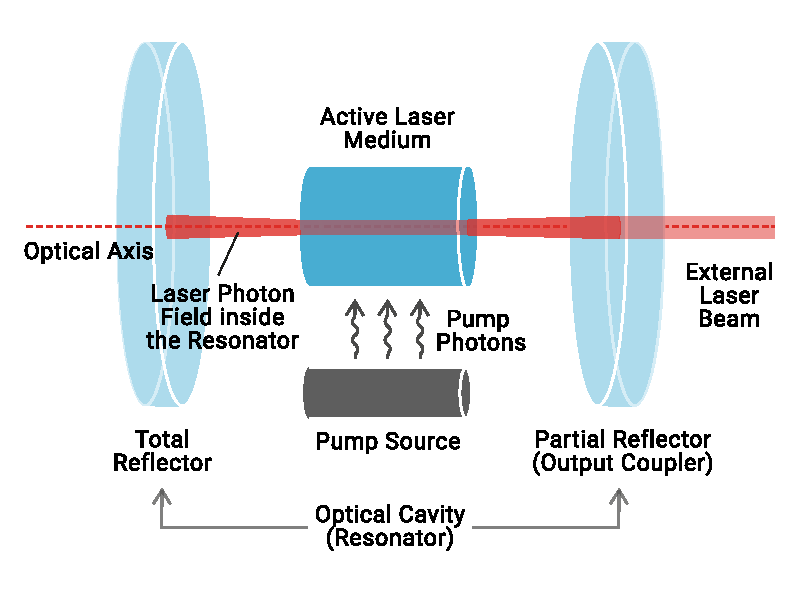
\includegraphics[width=0.75\linewidth]{planning/images/laser_gain.pdf}
	\caption{The components of a laser are depicted which include the pump source, active laser medium, and optical cavity. Image source: \cite{MeetOpticsPost}.}
	\label{fig:laser_gain}
\end{figure}

A typical laser operates by adding energy to some material, called the active lasing medium, from a pump source. The pump source can either be a strong flash of light or a pulse from a lower powered laser. The atoms in the medium absorb light which excites electrons to higher energy states. Over time, photons collide with excited atoms to stimulate emission of more photons. The medium is situated in an optical cavity (or resonator) composed of two reflecting mirrors that bounce these photons back and forth many times. With each reflection, photons pass back through the lasing medium, gaining more photon energy through stimulated emission as seen in \autoref{fig:laser_gain}. As a result, the active lasing medium is sometimes called the gain medium. Since one of the reflectors is only partially reflective, some of this laser light will pass through to become an external laser beam.

Lasers are best known for their ability to produce focused, high intensity light at a particular wavelength. Low powered lasers can be used as a laser pointer for a presentation, while higher powered lasers can cut solids. From both fundamental physics and industry perspectives, scientists are interested in increasing the intensity of lasers to explore various \gls{HEDS} phenomena. The most basic definition of intensity is

\begin{equation}
	\text{Intensity} = \frac{\text{Energy}}{\text{Area} \times \text{Time}}	
\end{equation}
So, for a given laser pulse, increasing the intensity could involve increasing the energy, decreasing the area (in terms of the surface that the laser beam hits), or decreasing the time. The energy can be increased by letting the laser stimulate emission of photons in the optical cavity with more passes. However, when the intensity in the cavity becomes too large, damage to the optical components (like the gain medium) can occur. In 1985, this problem was addressed by Donna Strickland and Gerard Mourou \cite{Strickland_1985_Optics} by first stretching an initial pulse in time before reaching the amplification stage in the gain medium. A stretched pulse can continue to gain energy while being sufficiently spread out (less intense) to not damage optical components as illustrated in 
\autoref{fig:cpa}. After amplification, the pulse is then compressed back into a shorter pulse. The clever use of gratings that separate light of different wavelengths allows pulses to easily be stretched and compressed in time. This method called \gls{CPA}, resulted in a nobel prize \cite{Nobel_2018}.

\begin{figure}
	\centering
	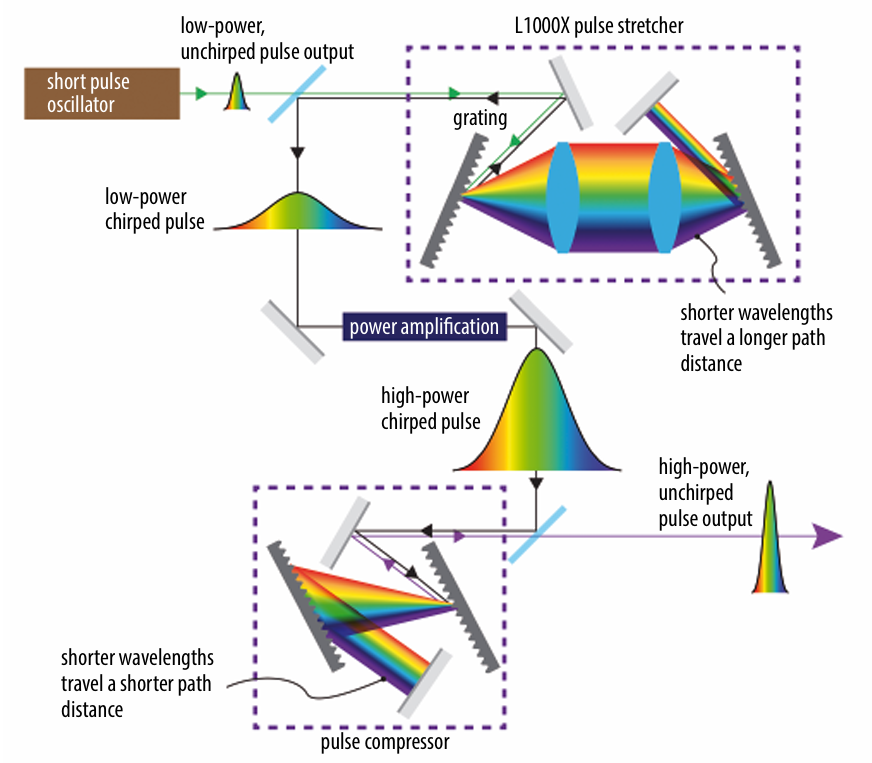
\includegraphics[width=0.9\linewidth]{planning/images/cpa.PNG}
	\caption{The stretch, amplification, and compression stages of chirped pulse amplification are depicted. Taken from \cite{Arrigoni_2019_Photonics}.}
	\label{fig:cpa}
\end{figure}
\gls{CPA} technology enabled lasers to produce high energy, extremely short femtosecond (a billionth of a millionth of a second) pulses that drove intensities into the relativistic regime where electrons can be accelerated to (nearly) the speed of light. The history of laser intensity since the production of the first laser in 1960 is depicted in \autoref{fig:laser_history}. The graph shows that between 1970-1985, laser intensities did not increase very much, but the invention of \gls{CPA} allowed intensities to increase 2-3 orders of magnitude every decade.

\begin{figure}
	\centering
	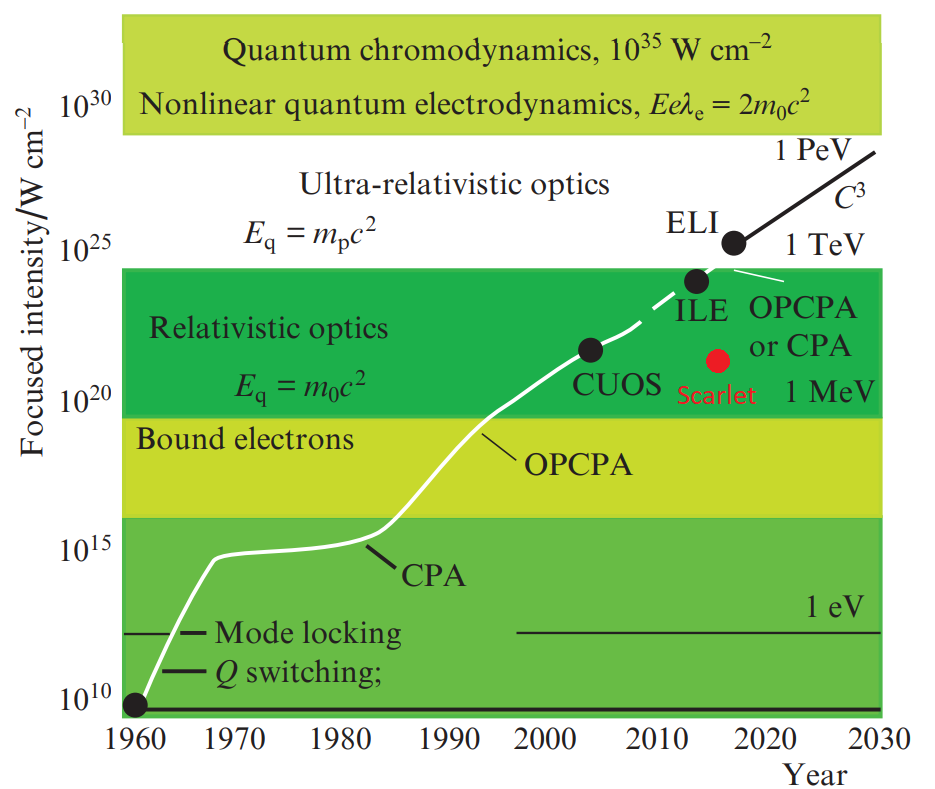
\includegraphics[width=0.75\linewidth]{planning/images/laser_history.PNG}
	\caption{History of focused laser intensities from the inception of the laser in 1960. The graph is labeled with intensity regimes, technological milestones, and acronyms of laser facilities. Modified from Figure 4 in Yakovlev \cite{Yakovlev_2014_QE} where OSU's Scarlet Laser was added.}
	\label{fig:laser_history}
\end{figure}

The laser at the Wright-Patterson Air Force base employs a titanium sapphire (Ti:Sapph) gain medium which is produced by doping (adding impurity) titanium ions in a sapphire\footnote{Corundrums are a mineral composed of aluminum oxide ($\text{Al}_2\text{O}_3$) with trace amounts of impurities that replace a small fraction of the aluminum ions. Blue sapphires have trace amounts of titanium and iron, while rubies have trace amounts of chromium.} crystal. These typically operate micron wavelength (infra-red) laser beams and are very commonly used in laser facilities across the globe. The Titan laser at \gls{JLF} uses a neodymium glass (Nd:glass) gain medium which is also configured for micron wavelengths. These two laser systems are the sites of the research discussed in this thesis.


\section{Applications}

The lasers described in the preceding section are used to study materials at high energy density scales. These laser-matter interactions are important for a variety of reasons. First, lasers can heat up materials to be as hot and dense as the core of the sun (if only for a tiny fraction of a second) which can provide astrophysical insights. Second, these hot, dense conditions are needed for nuclear fusion which is an extremely promising future source of clean energy (explored at places like the \gls{NIF}). Finally, laser-matter interactions can produce high energy, pulsed beams of protons, electrons, and ions. The most well-studied proton acceleration mechanism is called \gls{TNSA} whose physical origins will be explored more in \autoref{sec:acceleration}. 

During the course of my PhD, I have worked on ways to optimize the \gls{TNSA} mechanism for accelerating protons. This section highlights some of its most important applications: (1) proton therapy for cancer treatment, (2) proton radiography for imaging, and (3) ion beam analysis for materials characterization.


\subsection{Proton Therapy}

Cancer treatment is one of the largest medical challenges faced worldwide and cancer generally requires the use of harsh treatments like invasive surgery, chemotherapy, and immunotherapy. Another type of treatment is called radiotherapy and more than half of all people with cancer will receive it as a part of their medical care \cite{Mayo_2024_Cancer}. Typically, a large machine will provide a source of high energy x-rays that kills the tumor. However, this radiation does not discern whether the cells are cancerous or not -- healthy tissue along the radiation beam path surrounding the tumor will also be damaged. This damage can be mitigated by shooting many beams from different angles such that they overlap at the site of the tumor. In this way, the dose delivered in the beam overlap region will be significantly higher than the surrounding tissue. This approach is typically employed by situating the machine on a rotating ``gantry''.

As early as 1905, Bragg \cite{Bragg_1905_JOS} identified that charged particles have different properties than x-rays when passing through matter. Specifically, he identified that radium particles lost more energy (i.e. delivered a higher dose) at a lower speed. Physically, the slower the radium particles, the more time they have to scatter with individual atoms and the more energy they can deposit. This means that when radium first enters a material at its highest speed, it is losing energy slowly. In contrast, when radium is at a slow speed and about to stop, it is losing energy very quickly. In 1946, Wilson \cite{Wilson_1946_Rad} recognized that this property of charged particles could deliver a concentrated dose close to a tumor site. In \autoref{fig:bragg_curve}, these differences are explicitly highlighted between x-rays and proton beams traveling through water. It can be seen that the proton beam is sharply peaked at a distance of 24 centimeters, whereas the x-ray beam delivers a higher dose just a few centimeters in. One can see the advantage of protons quite readily from this picture -- if a tumor is located 24 centimeters into the body, the protons, comparatively to the x-rays, will deliver more energy at the tumor site and less energy to the surrounding tissue. Additionally, the dose delivered reduces to zero behind the tumor for protons which is not true for x-rays. The shape of the proton beam curve in this graph is appropriately referred to as a \emph{Bragg Curve} which peaks at the \emph{Bragg Peak}. 

The specifics of the depth-dose curve depend on the material that the particles are traveling through as well as initial energy of the protons (with higher energy protons traveling further into the material). These conditions are well-studied by empirical measurements of the \gls{SRIM} \cite{Ziegler_2010_SRIM} and can be combined with other techniques to achieve a depth-dose curve that not only peaks at different depths, but widens the region where the highest dose is delivered. The most modern form of proton therapy is called \gls{IMPT} whose intensities are modulated to optimally balance tumor dose and sparing of normal tissues \cite{Mohan_2022_PRO}. The first proton therapy center opened at the Loma Linda University Medical Center in California in 1990, but today there are more than 100 centers around the world (with more in the planning or construction stage) \cite{Mohan_2022_PRO}. 

\begin{figure}
	\centering
	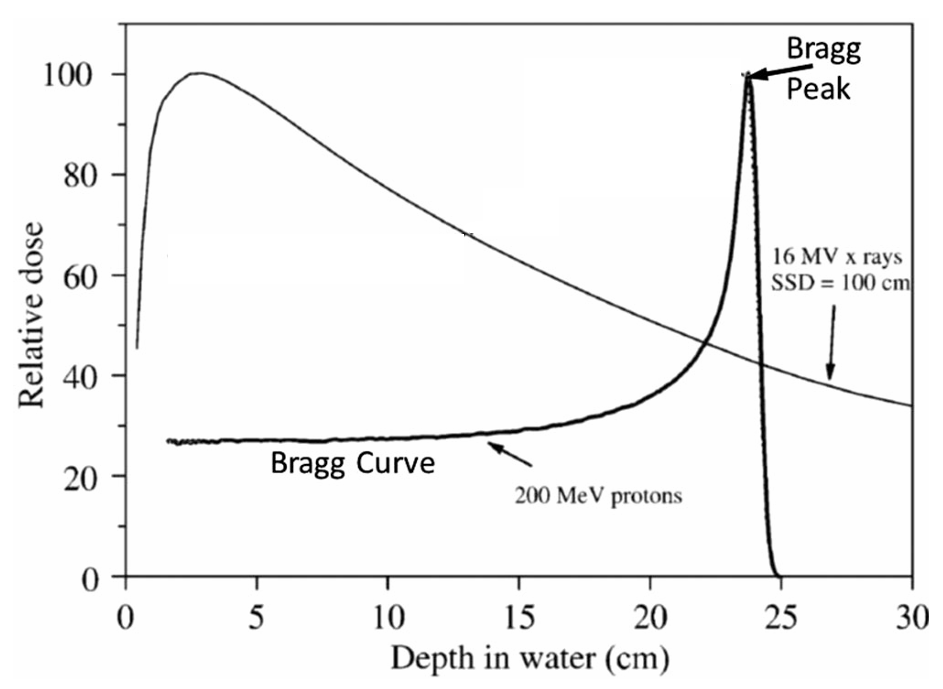
\includegraphics[width=0.75\linewidth]{planning/images/bragg_curve.PNG}
	\caption{The dose delivered as a function of depth traveled in water for two types of beams are depicted -- 200 MeV protons and 16 MV x-rays. Modified from Figure 1 in Mohan \cite{Mohan_2022_PRO}.}
	\label{fig:bragg_curve}
\end{figure}
 
Here in Columbus, \gls{OSUCCC}, in collaboration with Nationwide Children's Hospital, opened a 55,000 square foot proton therapy center in December of 2023 \cite{OSU_CCC} that uses \gls{IMPT}. Despite all the aformentioned benefits of proton therapy, the intial cost is tremendous -- \gls{OSUCCC} was a 100 million dollar investment. The significant cost demonstrates the value this could bring to Central Ohio. The facility is even outfitted with the capability to perform FLASH\footnote{Despite the capitalization, FLASH is not an acronym.} therapy which is a newer, experimental form of proton therapy. Compared to conventional methods, FLASH uses much higher dose-rates (i.e. greater than 40 Gy/s instead of less than 1 Gy/s) with much shorter exposure times (fractions of a second instead of minutes) for the same total dose. The higher dose-rate has been shown to reduce radiation-induced toxicity in healthy tissues in pre-clinical trials \cite{Matuszak_2022_Onc} and is currently under clinical trials \cite{OSU_CCC}. 

The conventional cyclotron accelerators used at \gls{OSUCCC} are extremely large and expensive which limits their availability to select locations globally. In recent years, it has been proposed that laser-based particle accelerators could be used to generate high energy protons. Laser-based sources can potentially produce even higher dose-rates ($\sim10^7$ Gy/s) and shorter exposure times (nanoseconds) for FLASH therapy \cite{Bin_2022_SciRep} to further reduce radiation-induced toxicity. Also, laser facilities could in principle be smaller and less costly. On the other hand, the technology is not matured enough to be considered in the near future \cite{Linz_2016_LaPB}. Current laser-based sources are typically only able to generate protons in the 10s of MeV reliably (as opposed to the 100s of MeV required for clinical operation) and exhibit poor repeatability of the laser pulse output. In addition, the conventional accelerators have already made significant strides in terms of reducing cost, increasing beam quality, and reducing size in recent years \cite{Linz_2016_LaPB} which is something laser-based sources will need to keep up with in the future. However, the potential of developing a smaller, lower cost, higher dose rate proton accelerator remains an important motivating factor for many laser-plasma physicists in the coming years.

\subsection{Laser Fusion and Proton Radiography}

Another use for protons is a diagnostic for laser fusion experiments. These use high powered lasers to compress a millimeter sized frozen pellet of hydrogen fuel\footnote{Specifically, heavier isotopes of hydrogen called deuterium and tritium are used} to such high temperatures and pressures similar to the core of the sun that the atomic nuclei fuse together into helium.

\begin{figure}
	\centering
	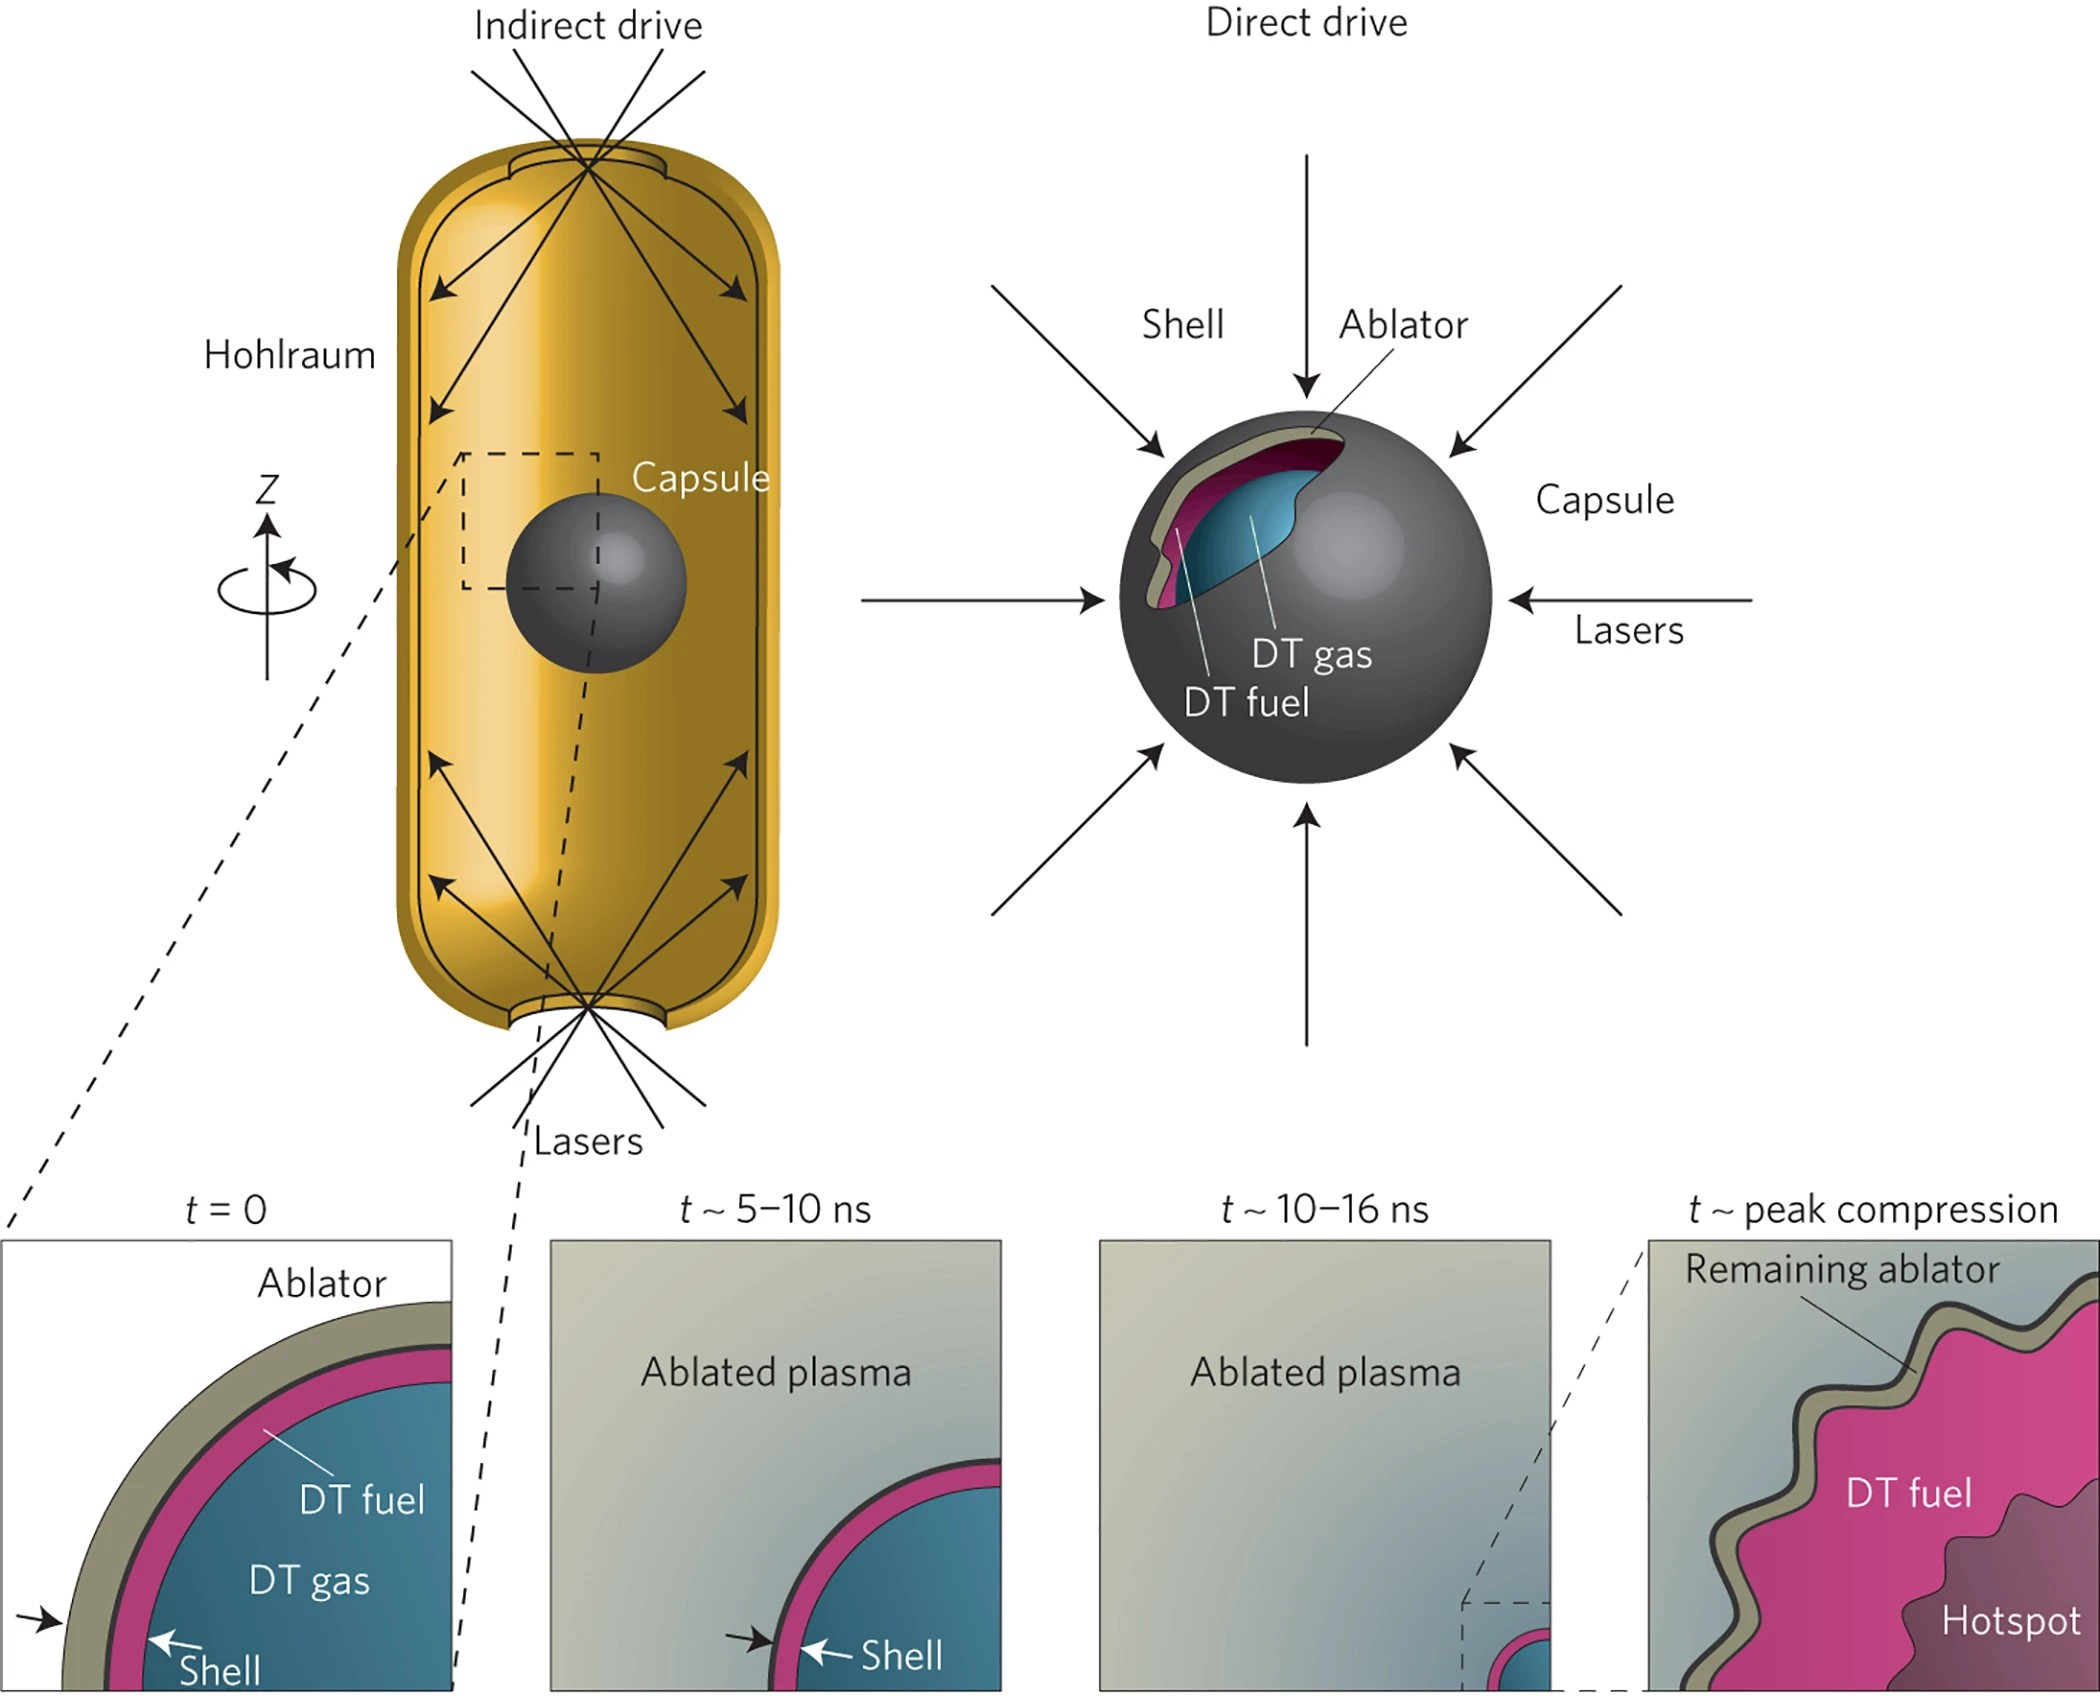
\includegraphics[width=0.9\linewidth]{planning/images/fusion.png}
	\caption{Visualization of two different approaches to laser fusion are depicted at the top. Lasers can irradiate the inside of a hollow gold can (called a hohlraum) to indirectly heat a fusion capsule or instead directly heat it. At the bottom, multiple stages of the fusion process are depicted including capsule ablation, compression, and burn. Taken from Figure 1 of Betti et al. \cite{Betti_2016_Nature}. }
	\label{fig:inertial_fusion}
\end{figure}

The fusion efforts are primarily conducted at two institutions in the United States. At the University of Rochester's \gls{LLE}, the OMEGA laser directly irradiates a fusion pellet in an approach called \emph{direct drive}. This is in contrast to the \gls{NIF} which indirectly compresses a fusion pellet by first irradiating a surrounding gold can in an approach called \emph{indirect drive}. These two approaches along with various fusion stages are illustrated in \autoref{fig:inertial_fusion}.

While visible light is typically used to image objects, other frequencies of light can be used as well. High frequency sources like x-rays are used at the dentist due to their ability to probe matter within your body. Radio waves reflect well off of electrically conductive materials like the metals in vehicles which make them ideal for military applications. Massive particles like protons can also be used and their different properties can be exploited to image things that cannot be done well with other types of radiation \cite{Schaeffer_2023_RevMod}. For example, the existence of the Bragg Peak in \autoref{fig:bragg_curve} enables proton images to have higher contrast than x-rays which deposit energy more uniformly.
 
For a laser fusion experiment with a nanosecond laser, an even shorter burst of protons would be needed to capture a ``still'' image or radiograph of the target at peak compression. Conventional sources of protons for radiography purposes are from linear accelerators like the pRad at \gls{LANL} that can accelerate up to 800 MeV protons \cite{LANL_PRAD} which can create microsecond or millisecond bursts of protons. In contrast, laser-driven proton sources can be generated in picosecond bursts through the \gls{TNSA} mechanism. Another advantage of these laser-accelerated proton beams is that they are emitted from a very small spot, on the order of microns, which is beneficial for obtaining a higher quality image \cite{Schaeffer_2023_RevMod}. This can be illustrated with a simple analogy to visible light -- the shadow produced from a small flashlight will have sharper edges than one produced from a larger fluorescent ceiling light.

With these considerations in mind, proton radiography has been demonstrated successfully at the \gls{NIF} through \gls{NIF-ARC} \cite{Simpson_2021_PPCF} and at OMEGA through \gls{OMEGA-EP} \cite{Zylstra_2012_RSI}. Both \gls{NIF-ARC} and \gls{OMEGA-EP} use a picosecond scale laser to produce \gls{TNSA} proton beams from laser-irradiated metallic foils and allow scientists to image fusion experiments on a timescale that would not be otherwise possible.

\subsection{Materials Characterization}

While protons can generate images through radiography, they can more generally tell us information about materials through a process called \gls{IBA}. \gls{IBA} allows scientists to probe material composition and surface structures with MeV ion beams which are appealing partly due to their non-destructive nature (comparatively to sources like x-rays) \cite{Passoni_2019_SciRep}. \gls{IBA} is currently implemented through old Van de Graaf and Tandem accelerator technology, but Passoni \cite{Passoni_2019_SciRep} argues that \gls{TNSA} proton beams can achieve the same result in a more compact, portable, and cheaper setup.

\begin{figure}
	\centering
	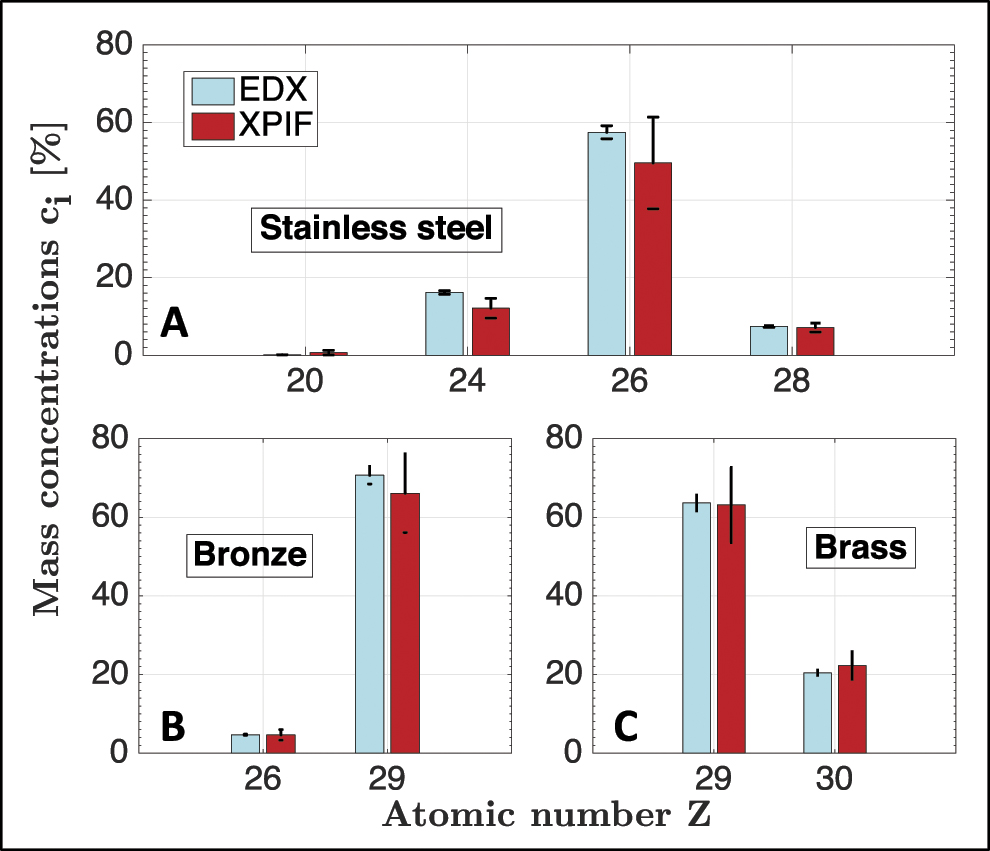
\includegraphics[width=0.6\linewidth]{planning/images/mass_concentration.jpg}
	\caption{Mass concentrations of three metal alloys are shown using two different techniques: Energy Dispersive x-ray Fluorescence (EDF) and X-ray and Particle-Induced Fluorescence. Taken from Figure 4 of Boivin et al. \cite{Boivin_2022_NJoP}.}
	\label{fig:mass_concentration}
\end{figure}

As a proof of principle, Boivin \cite{Boivin_2022_NJoP} used TNSA beams from the \gls{ALLS} laser facility in Canada to determine the elemental mass concentrations of three different metal alloys: stainless steel, bronze, and  brass using \gls{XPIF}. This is compared to a method called \gls{EDX} used in conjunction with a conventional mono-energetic electron beam and shown in \autoref{fig:mass_concentration}. Although XPIF has larger error bars than \gls{EDX}, both methods find good agreement with each other.

As a final point, \gls{TNSA} beams can be accompanied by other radiation sources like electrons, x-rays, and neutrons. Different materials characterization processes could, in principle, be used in conjunction with each other. While \gls{TNSA} beams are not the most common way to characterize materials today, they may emerge as an important tool for their ability to be pulsed at a high repetition rate and generated from a relatively compact system.

\section{Outline}
In the last decade, machine learning has emerged as an increasingly important tool\footnote{This is especially clear from the past few years of generative AI with tools like Chat-GPT.} for understanding the vast volume of data present in this world. Scientists have already been using machine learning in other fields to make new discoveries, but the field of laser-driven proton acceleration has only started to make use of it. This is because machine learning requires an immense amount of data to provide a true benefit \cite{Dopp_2023_HPLSE} and most modern laser systems only produce around one pulse per second (or less). Before my time, our group produced \gls{TNSA} proton beams in 2018 \cite{Morrison_2018_NJoP} from a laser system that sends 1000 pulses a second. With this many pulses, collecting large amounts of data now becomes a reality. However, to realize applications, the \gls{TNSA} proton beams need to be optimized for specific use cases. 

This work is a continuation of prior efforts in the group to computationally study \gls{TNSA} proton beams from Gregory Ngirmang, Joseph Smith, Nashad Rahman and others. In \autoref{ch:2} and \autoref{ch:3}, I give the physics and computational background needed to understand the main body of the dissertation. The bulk of my PhD work is summarized in \autoref{ch:5} which involved the construction of a synthetic proton acceleration dataset. This data was used as a testbed for assessing the feasibility of applying machine learning to possible future proton acceleration datasets. In \autoref{ch:4}, I detail the simulations I ran to corroborate the experimental findings of enhanced proton acceleration from the use of a split pulse. A future laser facility could possibility use the split pulse scheme as one of many optimizations to achieve a proton beam with desired properties. In \autoref{ch:6}, I detail my involvement in programming a machine learning feedback loop to automatically optimize accelerated electrons and protons from collected data. Finally, in \autoref{ch:7}, I conclude and give suggestions for future work.



\chapter{Laser-Plasma Interactions and Ion-Acceleration} \label{ch:2}

%\begin{table}
%\begin{center}
%\begin{tabular}{lll}
%\hline
%\\[3pt]
%Alphabet Character & Vowel & Number \\[3pt]
%\hline
%\\[3pt]
%A & Yes & 1 \\
%B & No & 2 \\
%C & No & 3 \\[3pt]
%\hline
%\end{tabular}
%\label{tbl3}
%\caption{Another Table}
%\end{center}
%\end{table}

\section{Plasma Physics}

Chen \cite{Chen_2015_Plasma} describes a plasma as

\begin{quote}
	a \emph{quasineutral} gas of charged and neutral particles which exhibits \emph{collective behavior}
\end{quote}
In this section, the quasineutrality and collective behavior of plasmas will be discussed. One way to create a plasma is through the interaction of matter with an energetic laser. The laser has enough energy to ionize atoms to a hot dense soup that satisfy the definition of Chen. Plasmas do exist in other contexts, like those found in stars and various astrophysical systems, but these will not be explained in detail in this section. Here, we'll overview the physics of gaussian laser beams, particle motions in electric fields, and the properties of plasmas.

% are found everywhere: Lightning, plasma etching, fusion energy. Magnetic and Inertial and Graviational Confinement. Polar aurorae, solar wind, ion thrusters.
%
%Even though one can think of a plasma as just an ionized gas, its properties thoroughly differentitate it from one. Gases typically rely on short-range collisions while plasmas involve collective motions of particles over a long-range due to the electrostatic forces. Gases have low conductivity, while plasmas have nearly infinite conductivity which allows for the high charge separation and high field strengths. Plasmas can also have multiple species that behave vastly differently (different mass/charge) which can result in different types of waves and instabilities.
%
%Plasmas are very similar to many metals in the fact that they both conduct electricity well. However, metals are solids and typically have worse conductivity at higher temperature, while plasmas conduct electricity well at high temps. 
%
%Can derive e field from boltzmann relation as E = kb T / e (del ne) / ne

\subsection{Gaussian Laser}
In order to heat up a material with a laser efficiently, the energy would ideally be concentrated to a small point. For example, the typical incandescent household light bulb radiates energy equally in all directions and does not do a good job of focusing energy to a point. But, using a magnifying glass can effectively concentrate the energy. For this reason, focusing optics play an important part in the field of plasma physics. 

However, to obtain a focused light source, we can use lasers that have the capability of producing narrow beams. The intended output of many lasers have an electric field described by the fundantal transverse electromagnetic mode \cite{Zangwill_2012} (TEM$_{00}$) described by the following electric field

\begin{equation}
	E(r, x) = E_0 \hat{y} \frac{w_0}{w(x)} \exp( - \frac{r^2}{w(x)^2}) \cos(k x - \arctan(x/x_R) + \frac{k r^2}{2 R(x)}) \label{eq:gaussian_beam}
\end{equation}
where $\hat{x}$ is the propagation direction, $\hat{y}$ is the polarization direction, and $r = \sqrt{y^2 + z^2}$ is the radial distance away from the laser axis. In the cosine function, $R(z) = z [1 + (z_R/z)^2]$ is the radius of curvature and $\arctan(z/z_R)$ is the guoy phase. For our purposes, these won't have too much relevance. Additionally, the beam radius $w$ is expressed as

\begin{equation}
	w(z) = w_0 \sqrt{1 + (z/z_R)^2} \label{eq:beam_radius}
\end{equation}  
and has a minimum value at the \emph{beam waist} $w(0) \equiv w_0$ at the focal position of the laser. The length scale over which the beam can propagate without diverging significantly is the \emph{Rayleigh range} $x_R \equiv \frac{\pi w_0^2}{\lambda}$. The peak intensity is related to the electric field by $I_0 = \frac{1}{2} \epsilon_0 c E_0^2$ and \cref{eq:gaussian_beam} shows that the intensity decays as $I(x, r) = I_0 (w_0 / w(x))^2 \exp(-2 r^2 / w(x)^2)$ with increasing $r$ and $x$. If we integrate this intensity distribution over the entire $y-z$ plane, we obtain the peak power $P_0 = \frac{\pi \omega_0^2}{2} I_0$. Furthermore, we can integrate the power over the pulse duration (assuming the pulse has a $sin^2(t)$ envelope) to obtain the total energy in the pulse 

\begin{equation}
	E = \frac{\pi \omega_0^2}{2} I_0 \tau_\text{fwhm} \label{eq:gaussian_beam_energy}
\end{equation}
where $\tau_\text{fwhm}$ is the full-width half-max and is equal to half the pulse duration for a $sin^2(t)$ pulse envelope. 

\subsection{Single Particle Motions}

Electrostatics is governed by the Maxwell's equations which describe the allowed wave-like solutions for electric and magnetic fields in both matter and vacuum. The most relevant equation in this section is Gauss' Law or Poisson's Equation which can be expressed as 

\begin{equation}
	- \nabla^2 \phi = \nabla \cdot \vec{E} \equiv \frac{\rho}{\epsilon_0} \label{eq:poisson}
\end{equation}
which relates the electrostatic potential $\phi$ or electric field $E$ to the charge density $\rho$. This equation highlights how electric fields are directed radially outward from positive charges and inward towards negative charges. The motion of an electron in the influence of an electric field $E$ or magnetic field $B$ is given by the \emph{Lorentz force} $F_L$

\begin{equation}
	F_L \equiv -e (\vec{E} + \vec{v} \times \vec{B}) \label{eq:lorentz}
\end{equation}

\subsubsection{Quiver Energy}
To gain intuition about some quantities of interest for laser-matter interactions, let's consider a simple problem of an electron of charge $-e$ governed by \cref{eq:lorentz} with a negligible magnetic field $B$. Additionally, only consider 1D motion in the oscillating field $E = E_0 \cos(\omega t)$ for a laser field of frequency $\omega$. Then, the equation of motion is

\begin{equation}
	\frac{d v}{d t} = - \frac{e E_0}{m} \cos(\omega t)
\end{equation}
We can integrate this equation to obtain the velocity and position as a function of time (assuming $x_0 = v_0 = 0$)

\begin{align}
	v(t) &= - v_\text{osc} \sin(\omega t) \label{eq:v(t)} \\
	x(t) &= \frac{v_\text{osc}}{\omega} [\cos(\omega t) - 1] \label{eq:x(t)}
\end{align}
where $v_\text{osc} \equiv (e E_0) / (m \omega)$ is defined as the \emph{quiver velocity}. From \autoref{eq:v(t)}, we can calculate the kinetic energy gained by an electron as $U_p \equiv \frac{1}{2} m \langle v^2 \rangle = \frac{1}{4} m v_\text{osc}^2$ which is known as the \emph{ponderomotive potential (energy)}. This energy represents the cycle-averaged quiver energy of an electron in an electromagnetic field. A more commonly used term is the dimensionless \emph{normalized vector potential} $a_0$ which is closely related to the quiver velocity

\begin{equation}
	a_0 \equiv v_\text{osc} / c = \frac{e E_0}{m \omega c} \label{eq:a0}
\end{equation}
Ultra-intense laser-matter interactions involve relativistic electrons which are produced when $a_0 \gtrsim 1$. In terms of the field, $a_0 \sim 1$ corresponds to a peak electric field $E_0 = \frac{2 \pi m c^2}{e \lambda} \simeq \SI{4}{\tera \volt \per \meter}$. In terms of the peak intensity, $I_0 = \frac{1}{2} c \epsilon_0 E_0^2 \simeq \SI{2e18}{\watt \per \centi \meter \squared}$ for this electric field. Consequently, the threshold for relativistic interactions is commonly understood as $I_0 \gtrsim \SI{1e18}{\watt \per \centi \meter \squared}$. 

\subsubsection{Ponderomotive Force}
The above approach yields some important scales for laser-matter interactions, but only describes the interaction of a plane wave that is spatially homogeneous. A real laser field would be spatially inhomogeneous and we can express $E(x) \approx E_0 + x E_0'(x)$ to first order. This modifies the equation of motion as 

\begin{equation}
	\frac{d v}{d t} = - \frac{e E_0}{m} \cos(\omega t) - \frac{e E_0'}{m} \cos(\omega t)[ \frac{v_\text{osc}}{\omega}(\cos(\omega t) - 1)]
\end{equation}
where we've inserted the expression for x from \cref{eq:x(t)} which should be approximately true for small $x$. This equation can be simplified and separated into oscillating and non-oscillating components as

% should maybe cite arefiev notes, not sure how, because I can't find it online.
\begin{equation}
	\frac{d v}{d t} = - \frac{e E_0}{m} [\cos(\omega t)(1 - \frac{E_0' v_\text{osc}}{e_0 \omega}) + \frac{E_0' v_\text{osc}}{2 \omega E_0} \cos(2 \omega t)] - \frac{e E_0' v_\text{osc}}{2 m \omega}
\end{equation}
Over many cycles, the oscillating components will average out to zero and the remaining term is given by $\langle F_p \rangle = m \frac{d v}{d t} = - \frac{e E_0' v_\text{osc}}{2 m \omega}$ and is called the \emph{ponderomotive force}. We can generalize this to 3D and express this time-averaged force in several different, equivalent ways

\begin{equation}
	\langle F_p \rangle = - \frac{e^2}{2 m \omega^2} \lvert E_0 \rvert \nabla E_0 = - \frac{m c^2}{4} \nabla(a_0^2) = - \nabla U_p \label{eq:pond_force}
\end{equation}
where 
\begin{equation}
	U_p = \frac{e^2 E_0^2}{4 m \omega^2} = \frac{1}{4} m v_\text{osc}^2 \label{eq:pond_potential}
\end{equation}
is the ponderomotive potential energy introduced earlier. 

The ponderomotive force is an important mechanism in the absorption of laser energy by electrons which will be expanded upon in \cref{sec:absorption}.

\subsection{Properties of a Plasma}
The quasi-neutrality condition reflects the fact that a plasma is charge neutral throughout its volume in a similar way to an ideal conductor: mobile electrons will reorganize themselves in the presence of an external electric field to maintain zero field (or constant  potential). The simplest plasma description will assume the ions are immobile (due to being much heavier than the electrons) and can be treated as a constant neutralizing background density $n_i$ for the electrons of density $n_{e,0} = Z n_i$ (for a plasma with atomic number $Z$).

\begin{figure}
	\centering
	\includegraphics[width=0.75\linewidth]{planning/images/plasma_oscillation.PNG}
	\caption{An initially charge-neutral plasma is depicted on the left. On the right, the electrons are displaced by a distance $x$ creating a charge separation and electric field akin to a parallel-plate capacitor directed towards the right. Adapted from Smith \cite{Smith_2020_Thesis}.}
	\label{fig:plasma_oscillation}
\end{figure}

\subsubsection{Plasma Electron Oscillations}
A simple example can be illustrated by \cref{fig:plasma_oscillation} which shows a sheet of negative charge density $-\sigma = -e n_e x$ displaced to the right a small distance $x$. The region in the bulk of the plasma will experience a force from the parallel plate ``capacitor'' fields directed to the left.

\begin{equation}
	F = m \frac{d^2 x}{d t^2} = - e \frac{e n_e x}{\epsilon_0}
\end{equation}
which has the form of a restoring force that brings the charge imbalance back to the center of the plasma. This oscillatory motion has an associated frequency 

\begin{equation}
	\omega_{p,e} = \sqrt{\frac{n_e e^2}{m_e \epsilon_0}} \label{eq:omegape}
\end{equation}
that gives the timescale for electron motion in the plasma. This characteristic frequency shows why plasmas support collective motion (in opposition to a neutral gas in which collisions between individual particles only happen). To get a feeling for this timescale, let's assume a somewhat typical electron density \SI{1e29}{\per \meter \cubed} in laser-plasma interactions to yield a timescale of $\omega_{p,e}^{-1} \simeq \SI{0.1}{\femto \second}$.

Naturally (without externally imposed forces), these fluctuations in charge would be caused by thermal motions of electrons with a characteristic speed $v_{th}$ 

\begin{equation}
	v_{th} = \sqrt{\frac{k_B T_e}{m}} \label{eq:vthermal}
\end{equation}
Due to the strong restoring force from the charge separation, the electrons can only move a short distance $\lambda_D$, called the Debye length, out of equilibrium in this timescale. We can estimate this length by equating $v_{th} = \lambda_D / t \simeq \lambda_D \omega_{p,e}$ and solve for $\lambda_D$.

\begin{equation}
	\lambda_D = \frac{v_{th}}{\omega_{p,e}} = \sqrt{\frac{\epsilon_0 k_B T_e}{n_e e^2}} \label{eq:debye}
\end{equation} 
Physically, $\lambda_D$ gives a length scale over which the electrostatic force persists in a plasma. Within a distance $\lambda_D$ from some perturbation, charges will feel a force, and outside this distance, the charges will be completely shielded like that of an ideal conductor. 

\subsubsection{Fluid Model}
This description of a plasma as a sea of electrons with collective motion that allows wave-like motions naturally lends itself toward a fluid model. The first component of this model stems from \cref{eq:lorentz} whose explicit time and space dependence can be expressed through $\frac{d p}{d t} = m (\frac{\partial v}{\partial x} \frac{\partial x}{\partial t} + \frac{\partial v}{\partial t}) = m (\frac{\partial v}{\partial t} + v \frac{\partial v}{\partial x})$ (just considering one spatial dimension for simplicity). The second component of this model is the effect of the pressure gradient from thermal motions. Particles will tend to migrate from areas of higher pressure to lower pressure, where the thermal pressure is typically given by the familiar ideal gas law equation of state $p = n_e k_B T_e$. Consequently, the equation of motion should have a term that is opposite to the pressure gradient direction (i.e. $- \nabla p$). Combining these two components together in a generalized 3D equation results in

\begin{equation}
	m n_e (\frac{\partial \vec{u}}{\partial t} + (\vec{u} \cdot \nabla) \vec{u}) = -e n_e (\vec{E} + \vec{u} \times \vec{B}) - \nabla p \label{eq:fluid}
\end{equation}
where we've changed the single particle velocity $\vec{v}$ to the fluid velocity $\vec{u}$ and multiplied by the electron density $n_e$ to ensure correct units with the pressure gradient term. Then, let's look for a simple radially symmetric solution where the fluid velocity $u = 0$, magnetic field $B$ is negligible, and the temperature is constant (isothermal). Then, 

\begin{equation}
	n_e e E = - k_B T_e \frac{\partial n_e}{\partial r}
\end{equation}
and by relating the electric field to the potential $E = - \frac{dV}{dx}$, this equation can be integrated from $n_{e,0} \rightarrow n_e$ and $0 \rightarrow \phi$ to obtain 

\begin{equation}
	n_e = n_{e,0} \exp(\frac{e \phi}{k_B T_e}) \label{eq:boltzmann}
\end{equation}
which is referred to as the \emph{Boltzmann relation} for electrons \cite{Chen_2015_Plasma}. We can get an approximate solution to this equation when the potential $\phi$ is only slightly larger than the equilibrium $\phi=0$, which can be found when $e \phi << k_B T_e$. We can Taylor expand the density to obtain 

\begin{equation}
	n_e \approx n_{e,0}(1 + \frac{e \phi}{k_B T_e})
\end{equation} 
and if we assume a fully ionized plasma with immobile ions of charge $Z$, the density of ions satisfies $n{e,0} = Z n_i$ and \cref{eq:poisson} becomes 

\begin{equation}
	\epsilon_0 \nabla^2 \phi = - e n_{e,0} + e n_e = e n_{e,0} [1 + \frac{e \phi}{k_B T_e} - 1] = \frac{e^2 n_{e,0} \phi}{k_B T_e}
\end{equation}
This equation admits solutions of an exponentially decaying potential

\begin{equation}
	\phi(r) = \frac{Q}{r} \exp(-\frac{r}{\lambda_{D}}) \label{eq:shielding}
\end{equation}
where $\lambda_D = \sqrt{\frac{\epsilon_0 k_B T_e}{n_{e,0} e^2}}$ is the Debye length from \cref{eq:debye}. A visualization of the decaying potential from \cref{eq:shielding} is shown in \cref{fig:debye}. Looking at the center panel, we can see the fields drop off quickly within a distance $\lambda_D$ in contrast to the left panel's potential that extends much further out in distance $r$. The exponentially decaying potential is a feature of plasmas and highlights the ability of plasma electrons to shield fields in a distance $\lambda_D$. 

\begin{figure}
	\centering 
	\includegraphics[width=\linewidth]{planning/images/debye_length.png}
	\caption{Visualization of the electric potential as a function of radial distance away from a positive point charge at the origin in three scenarios: vacuum (left), plasma (center), ideal conductor (right). Brighter colors show a higher value of $\phi$. In the center panel, the debye length $\lambda_D$ is shown.}
	\label{fig:debye}
\end{figure}

\subsubsection{Plasma Conditions}
Putting all this together, we can define several conditions that must be satisfied for a plasma \cite{Chen_2015_Plasma}. Quasi-neutrality dictates that the plasma should be largely charge neutral. The only regions that aren't charge neutral are those that fall within $\lambda_D$ of some charge imbalance. Therefore, if $L$ is the length scale of the system in which the plasma resides, we require that $\lambda_D \ll L$. However, this condition is not sufficient because an ideal conductor has $\lambda_D = 0$ but is not a plasma due to the absence of collective behavior. Collective behavior can be enforced by asserting that there are enough electrons $N_D$ within a spherical volume of radius $\lambda_D$. The corresponding equation is $N_D = n_e (\frac{4}{3} \pi \lambda_D^3) \gg 1$. The final condition is that electrostatic interactions should dominate over collisions because the collective behavior (e.g. plasma oscillations) originates from the electrostatic forces. This means that the period of oscillations ($\omega_{p,e}^{-1}$) should be less than the mean time between collisions. 

\subsection{Absorption of Energy} \label{sec:absorption}

In order for a laser to couple energy to the plasma electrons, some absorption mechanism needs to take place. The most obvious way that electrons can gain energy is through collisions with other energetic electrons and ions. However, the collision frequency is known to get smaller as the temperature goes up \cite{Gibbon_2005_Plasma}, so much so that plasmas can be treated as collisionless for ultra-intense laser experiments. Below, some of the most common known heating mechanisms are summarized.

\subsubsection{Critical Density}
First, we will look at how the electric field from an oscillating electric field penetrates a plasma. Using \cref{eq:faraday,eq:ampere} combined with the vector identity $\nabla \times (\nabla \times \vec{E}) = \nabla(\nabla \cdot \vec{E}) - \nabla^2 \vec{E}$ \cite{Zangwill_2012}, we can solve for the vector wave equation in terms of only $\vec{E}$. 

\begin{equation}
	(\nabla^2 - \frac{1}{c^2} \frac{\partial^2}{\partial t^2}) \vec{E} = \mu_0 \frac{\partial J}{\partial t} + \nabla(\nabla \cdot \vec{E}) \label{eq:vectorwave}
\end{equation}
We can look for solutions of $\vec{E} = E(x) \cos(\omega t) \hat{x}$ that vary spatially only in the x direction. We are assuming $E(0)$ is the amplitude of the electric field at the boundary between vacuum $x < 0$ and matter $x > 0$ and wish to understand the form of $E(x)$ when $x > 0$. To proceed, we can assume the current density can be related to the drift velocity \cite{Macchi_2013_Plasma} by $J = -n_e e u$ where $u$ is the electron fluid velocity that satisfies \cref{eq:fluid}. Ignoring $B$ and thermal pressure, this relationship becomes 

\begin{equation}
	\frac{\partial \vec{J}}{\partial t} = \frac{n_e e^2}{m} E = \omega_p^2 \epsilon_0 \vec{E}
\end{equation}
using \cref{eq:omegape} which can be combined with \cref{eq:vectorwave} to obtain a differential equation for the electric field

\begin{equation}
	[\nabla^2 + \frac{\omega^2}{c^2}(1 - \frac{\omega_p^2}{\omega^2})] \vec{E} = 0
\end{equation}
By just focusing on the x-dependence, we can simplify this equation to 

\begin{equation}
	\frac{d^2 E}{d x^2} = \frac{1}{l_s^2}  E
\end{equation}
where $l_s^2 \equiv \frac{c^2}{\omega^2 - \omega_p^2}$ defines the \emph{skin depth} $l_s$. In the case where $\omega < \omega_p$, $l_s^2$ is negative and the solution has a sinusoidal dependence

\begin{equation}
	E(x) = E(0) \cos(x / l_s)
\end{equation}
On the other hand, when $\omega > \omega_p$, $l_s^2$ is positive and the solution has an exponential dependence

\begin{equation}
	E(x) = E(0) \exp(-x / l_s)
\end{equation}
where $l_s \equiv c / \omega_p$ is defined as the \emph{skin depth}. This ``evanescent'' behavior when $\omega > \omega_p$ occurs because the electrons cannot respond fast enough to the higher frequency $\omega$. Since the field cannot propagate effectively for $x > 0$, the plasma ends up reflecting a significant portion of the light. Since wavelength (and frequency) is fixed from the laser, we can reformulate this finding in terms of electron density. The critical density $n_c$ is defined as the electron density where $\omega = \omega_{p,e}$. Using \cref{eq:omegape}, this can be expressed as

\begin{equation}
	n_c \equiv \frac{m \epsilon_0}{e^2} \omega^2 \label{eq:criticaldensity}
\end{equation}
When $n_e > n_c$, the plasma is said to be \emph{overdense} and most of the laser light gets reflected. When $n_e < n_c$, the plasma is said to be \emph{underdense}, and the laser light can propagate through the plasma. 

A typical Ti:Sapphire laser has a wavelength of $\SI{0.8}{\micro \meter}$ which corresponds to a critical density of $n_c \simeq \SI{1.7e27}{\per \meter \cubed}$. In this work, two materials are of interest: gold and ethylene glycol which have densities of $\SI{19.3}{\gram \per \centi \meter \cubed}$ and $\SI{1.11}{\gram \per \centi \meter \cubed}$ respectively. These mass densities correspond to a number density of electrons $\SI{5.9e28}{\per \meter \cubed}$ and $\SI{1.1e28}{\per \meter \cubed}$ respectively assuming a singly ionized plasma. If the plasmas were multiply ionized, these densities would be even higher. Even though these ``solid density'' plasmas are clearly overdense, experiments show energy is able to efficiently couple to the electrons. Consequently, there must exist mechanisms of absorption that are consistent with the fact that most of the laser energy can only be deposited in a small depth $l_s$ into the plasma. 

\subsubsection{Resonance Absorption}
The previous discussion applied to an electric field directed in the x-direction. For gaussian laser beams, the electric field is always perpendicular to the direction of propagation. So, if the laser beam is to be directed toward a target at $x = 0$, normal incidence would imply that the electric field $E_x = 0$. Additionally, an s-polarized beam would have an electric field only in the z direction. As a result, the typical model of a laser beam depositing energy into a plasma involves a p-polarized laser beam traveling obliquely in the $x-y$ plane with some angle of incidence $\theta_i$ measured with respect to the normal direction of the target. Physically, plasma oscillations occur through fluctuations in density which are going to be the strongest in the x direction due to the interface between vacuum and matter.

Furthermore, Kruer \cite{Kruer_2003_Plasma} argues that the reflection of light at oblique incidence occurs at a density $n_e = n_c \cos^2(\theta_i)$ by enforcing momentum conservation of the electric field component in the $y$ direction. Even though we've discussed density profile as an abrupt step: from 0 to $n_e$ from crossing $x = 0$, an actual experiment would see some pre-heating of the target before the target becomes ionized and behaves as a mirror at the critical density. This can be characterized by some scale length $L_p \equiv n_e (\frac{\partial n_e}{\partial x})^{-1}$ which is smaller for steeper density profiles. As a result, at higher incidence angles, the evanescent portion of the electric field has to travel further into the underdense region of the target to reach the critical density. 

When the frequency of the laser $\omega \simeq \omega_p$, the laser light is in resonance with the plasma oscillations and the energy can be most efficiently absorbed. To maximize the amount of energy reaching the critical density surface in resonance, we would want $\theta_i$ to be large so that the electric field has a significant component in the $x$ direction, but also small enough so that the field doesn't diminish too much by traveling in the evanescent underdense region. Denisov \cite{Denisov_1957_JETP} and others \cite{Forslund_1975_PRA, Freidberg_1972_PRL, Estabrook_1975_PoF} addresses this question and develops a model for this so-called \emph{resonance absorption} An approximate version of this formula is given by Kruer \cite{Kruer_2003_Plasma}

\begin{equation}
	\phi(\tau) \simeq 2.3 \tau \exp(-2 \tau^3 / 3)
\end{equation}
where $\tau \equiv (k L_p)^{1/3} \sin(\theta_i)$ takes into account both the scale length and incidence angle. \cref{fig:absorption} shows the fractional absorption $\phi(\tau)^2/2$ of the incident light from this model as a function of $\theta_i$ for various scale lengths.There is an optimal angle $\theta_{max} \approx \arcsin(0.8 (k L_p)^{-1/3})$ that maximizes the absorption fraction (although Kruer notes that his simple model overestimates the peak absorption -- the  fraction should peak at around 0.5 \cite{Kruer_2003_Plasma}). 

\begin{figure}
	\centering 
	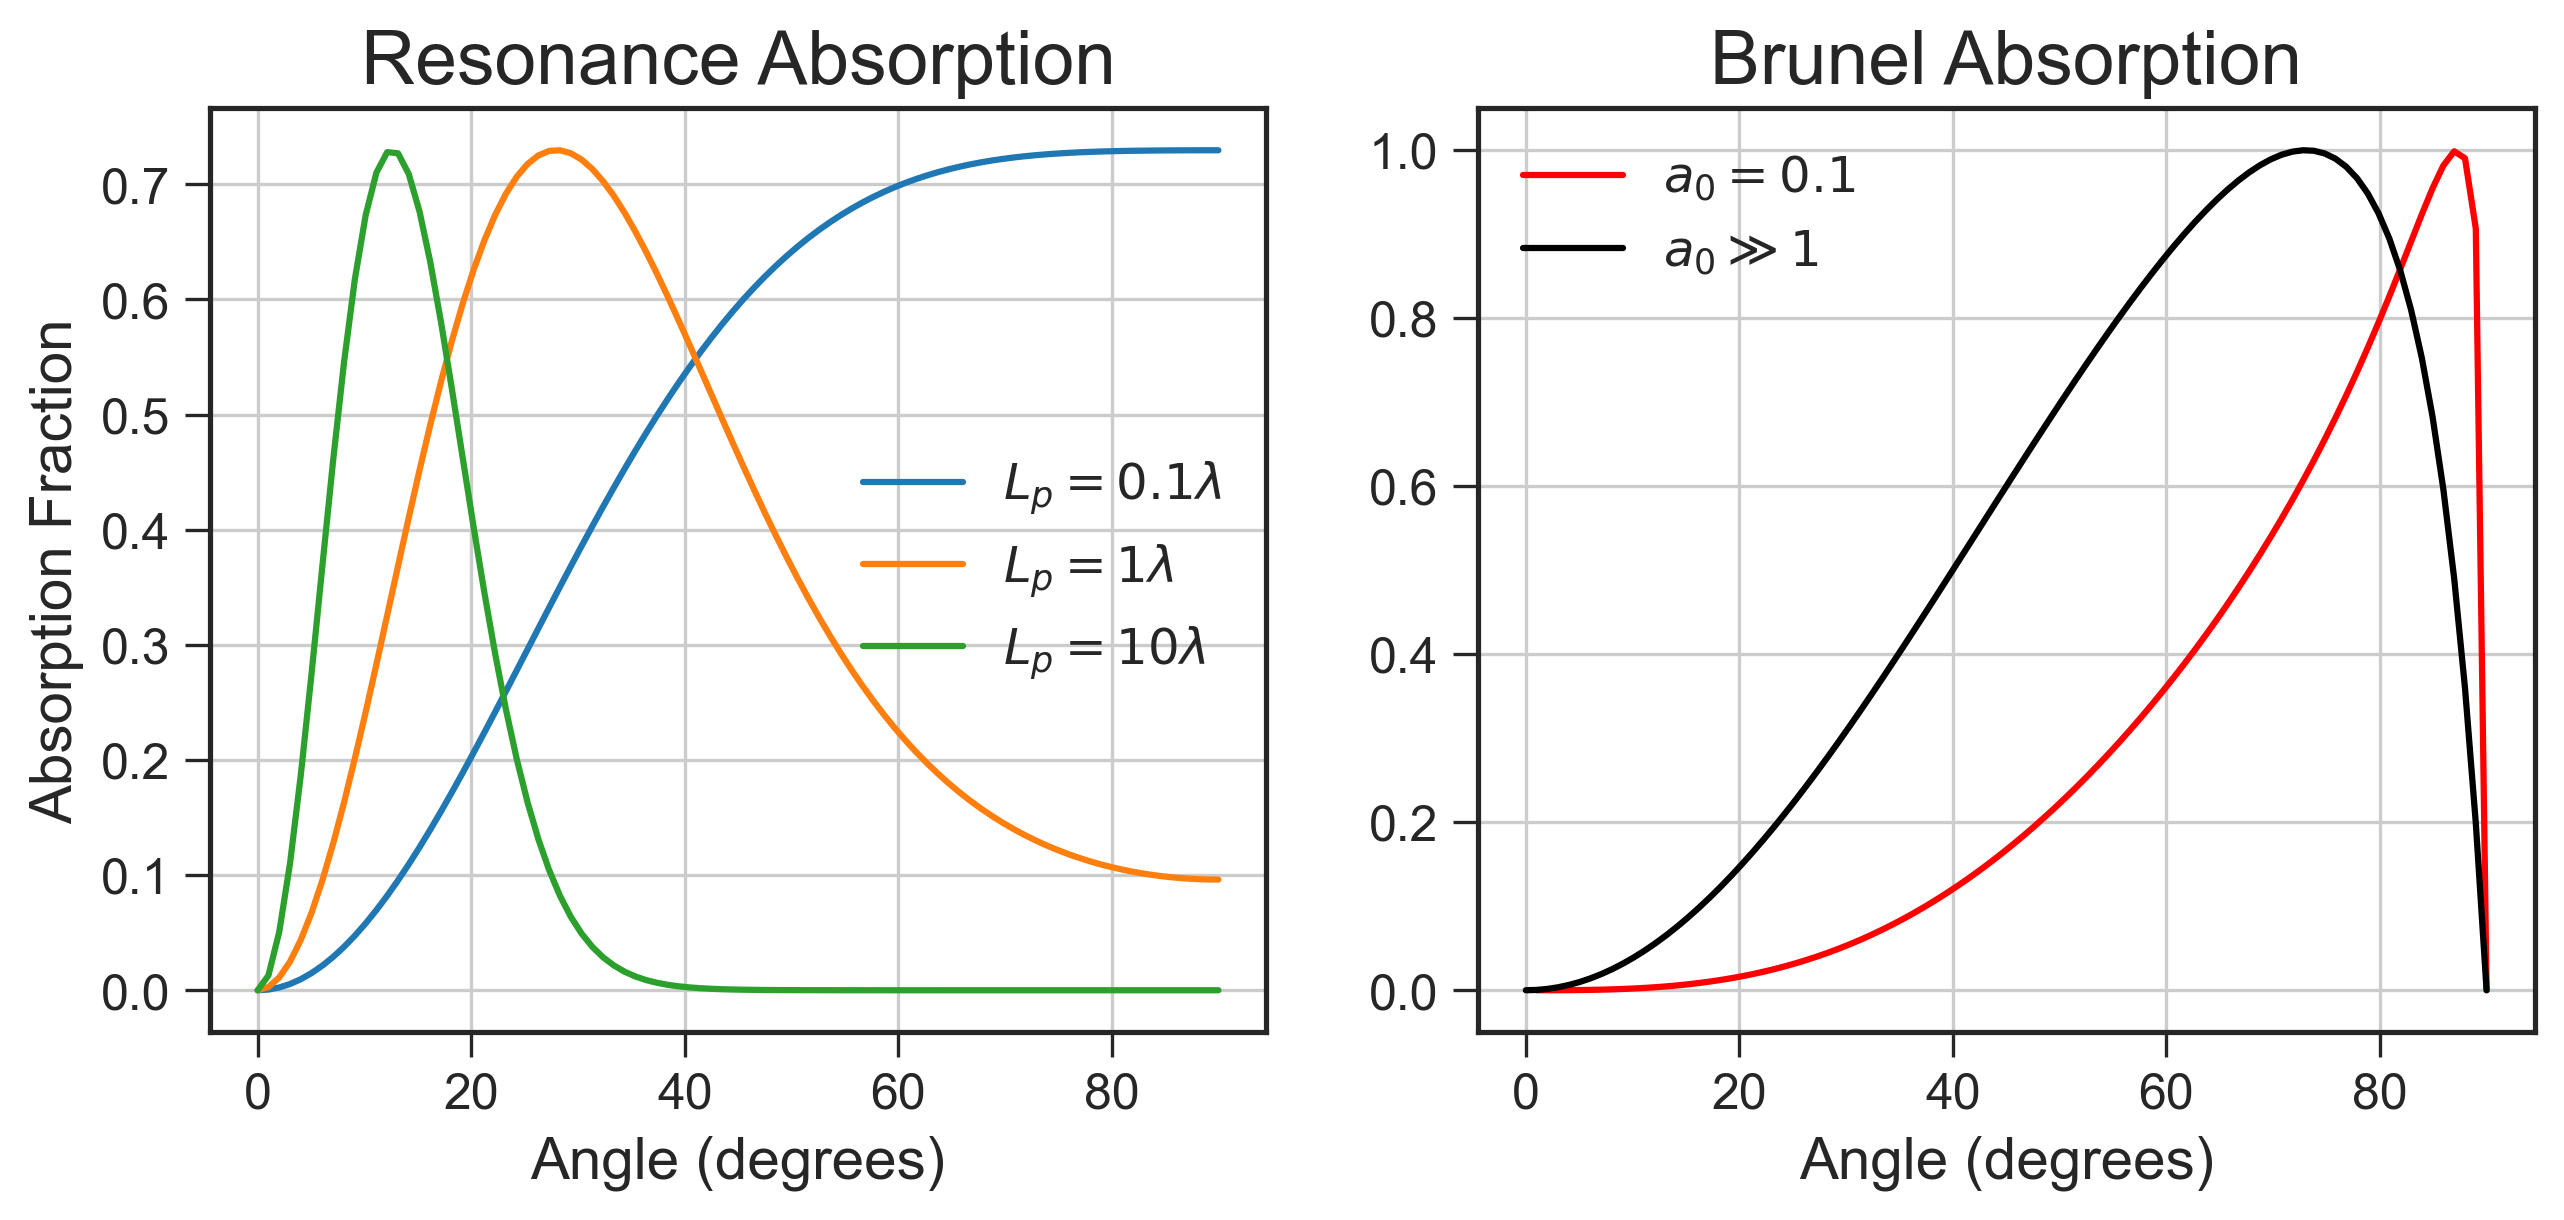
\includegraphics[width=\linewidth]{planning/images/absorption.png}
	\caption{Absorption fraction as a function of incidence angle $\theta_i$. For resonance absorption, the density scale length $L_p$ is varied in terms of the laser wavelength $\lambda = \SI{0.8}{\mu \meter}$. For the Brunel mechanism, fractions are plotted for two regimes $a_0 \ll 1$ (where a value of $a_0 = 0.1$ was chosen) and for $a_0 \gg 1$ (which has no dependence on $a_0$).}
	\label{fig:absorption}
\end{figure}

\subsubsection{Brunel Heating}
Resonance absorption only makes sense when the amplitude of the plasma oscillations $x_\text{osc} = v_\text{osc} / \omega = \frac{a_0 \lambda}{2 \pi}$ is less than the scale length $L_p$ \cite{Gibbon_2005_Plasma}, otherwise there is not enough available space for the oscillations to take place. For $\lambda = \SI{0.8}{\mu \meter}$ and $a_0 = 1$, $x_\text{osc} = \SI{127}{\nano \meter}$. However, for extremely small scale-lengths, efficient electron heating can still be observed \cite{Grimes_1999_PRL}. Consequently, a different type of heating mechanism is responsible in this case (somewhat confusingly) called ``not so resonant, resonant absorption'' \cite{Brunel_1987_PRL}. This model, developed by Brunel, is also known as \emph{vacuum heating} and will be explained below. 

Before explaining the Brunel mechanism, I should the basics of the 3-step model used for high-harmonic generation \cite{Corkum_1993_PRL}. Readers may find this model more familiar due to the recent 2023 Nobel Physics Prize won by Ohio State's Pierre Agostini \cite{Nobel_2023} which utilized the ideas of this model to produce attosecond pulses. This model involves a strong oscillating electric field $E(x) = E_0 \cos(\omega t)$ incident on an atom. Now, assume an electron is ionized at $t = t^*$. Under the influence of the oscillating field, the (initially stationary) electron will gain  and lose energy by moving away from the atom and returning back toward the atom. When $t^* \neq n \pi$ for integer $n$, it is actually possible for the electron to return back to the atom with non-zero energy. In fact, when $\omega t^* \approx 17^\circ + n (180^\circ)$, the electron returns with an energy peaking at $3.17 U_p$ where $U_p$ is the ponderomotive potential given by \cref{eq:pond_potential}. Furthermore, modeling the ionization rate through quantum-mechanical tunneling of an electron through a Coulomb potential warped by the oscillating laser field, we also determine that the most probable energy for an electron is strongly peaked at the $3.17 U_p$ cutoff. In short, this model shows how a laser field can produce electrons with energy on the scale of the ponderomotive potential with high probability at a frequency of twice per optical cycle. 

In the Brunel mechanism \cite{Brunel_1987_PRL}, we are considering a laser field incident on a planar target at $x > 0$ and vacuum at $x < 0$. In order for the electrons to escape the target, there needs to be some component of the electric field in the $x$ direction. Thus, we need to consider oblique incidence and p-polarization just like with resonance absorption. When the plasma scale length is small, the electrons will be able to travel far enough in the $x < 0$ to escape the plasma entirely and gain energy on the order of $U_p$ in a similar fashion to Corkum's model \cite{Corkum_1993_PRL}. Electrons arriving back to the target at just the right time will penetrate deeper than the skin depth $l_s \approx c / \omega_p$ and be inaccessible to the laser field \cite{Gibbon_2005_Plasma}. These \emph{hot electrons}, generated primarily on the front surface of the target, will provide the energy to heat the remainder of the overdense region of the target that the laser field cannot directly access. 

As mentioned, the optimal angle would appear to be for grazing incidence ($\theta_i = 90^\circ$), but Gibbon notes that accounting for imperfect reflection of the laser field and relativistic energies of the electrons, the efficiency no longer diverges at $\theta = 90^\circ$ \cite{Gibbon_2005_Plasma}. In \cref{fig:absorption}, some estimates for the absorption efficiency are plotted according to a simplified model developed by Gibbon \cite{Gibbon_2005_Plasma} based on Brunel \cite{Brunel_1987_PRL}.

\subsubsection{Other Mechanisms}
When the laser field penetrates a distance $l_s \approx c / \omega_p$ into the overdense region of the target, the electrons can heat up through collisions at an absorption rate $\eta \propto \frac{\nu_{ei}}{\omega_p,i}$ \cite{Gibbon_2005_Plasma} where $\nu_{ei}$ is the electron-ion collision frequency. This type of absorption is called the \emph{skin effect}. In this case, we see Fresnel-like reflection and absorption (see \cite{Griffiths_2017}) that is effective for large incidence angles. Even when the collision frequency is low, we can still get efficient absorption as long as the thermal electron motions are large compared to the skin depth (i.e. $v_{th}/\omega > l_s$) \cite{Gibbon_2005_Plasma}. This phenomena is called the \emph{anomalous skin effect} that is also most effective at large incidence angles. 

All of the mentioned phenomena work best at oblique incidence in p-polarization. But, for relativistic intensities, additional heating mechanisms arise. When $a_0 \gtrapprox 1$, the magnetic portion of \cref{eq:lorentz} becomes significant. At normal incidence, the electric and magnetic field components both fall in the $y-z$ plane. The electric fields move the electrons strongly causing a current $\vec{J}$ which in turn will interact with the laser magnetic field $\vec{B}$ in the direction perpendicular to both. As a result, this type of heating is known as $\vec{J} \times \vec{B}$ heating \cite{Gibbon_2005_Plasma,Kruer_1985_PoF}. Because $\vec{J} \times \vec{B}$ is in the direction of propagation, this effect is most pronounced at normal incidence. (TALK ABOUT HOW CIRCULAR POLARIZATION NEGATES JXB HEATING)

At even higher intensities, the laser can directly impart energy to the electrons through radiation pressure \cite{Macchi_2013_RevModPhys} because photons themselves carry momentum. These mechanisms are explored further in \cref{sec:acceleration}. In reality, all experiments involve a combination of several different electron heating mechanisms. Consequently, many experiments and simulations have been devoted to parametric studies that show how parameters ($L_p$, $\theta_i$, polarization, $a_0$, etc.) affect electron absorption(CITATION NEEDED)

\section{Ion Acceleration} \label{sec:acceleration}

The previous section gave an overview of the laser-plasma interactions and how they can efficiently couple energy into hot electrons. Regardless of heating mechanism, one theme is common to all -- the energy gained by an electron's quiver motion in an oscillatory field, known as the ponderomotive potential (\cref{eq:pond_potential}) sets the scale for the hot electron temperature $T_h$. That equation was only valid for non-relativistic electrons, so we must replace $U_p = \frac{1}{4} m v_\text{osc}^2$ with the relativistic kinetic energy $U_p \equiv (\gamma - 1) m c^2$ where $\gamma = 1 / \sqrt{1 - \frac{v_\text{osc}^2}{c^2}}$ defines the lorentz factor. We can combine this with the relativistic momentum $p = \gamma m v_\text{osc}$ and \cref{eq:a0} to determine an approximate expression of $\gamma$ in terms of $a_0$
	
\begin{equation}
	\gamma \simeq \sqrt{1 + a_0^2} = \sqrt{1 + \frac{I_{18} \lambda_{\mu m}^2}{1.37}} \label{eq:gamma}
\end{equation}
where $I_{18}$ is the peak intensity of the laser pulse in $\SI{1e18}{\watt \per \centi \meter \squared}$ and $\lambda_{\mu m}$ is the wavelength in $\mu m$. In 1992, Wilks \cite{Wilks_1992_PRL} conducted simulations to show that $T_h$ is on the order of $U_p$. 

\begin{equation}
	k_B T_h = m c^2 (\gamma - 1) \label{eq:wilks}
\end{equation}
In \cref{fig:electron_scaling}, we can see that the \emph{Wilks scaling} (pink) closely matches ultra-intense laser experiments. The other scalings in the figure are similarly validated by computational simulations and are all proportional to $(I \lambda^2)^\alpha$, where $0 < \alpha \leq 1$. As a result, the product $I \lambda^2$ is an important quantity in laser-plasma experiments and is called the \emph{irradiance}. Wilks also outlines a way to measure the hot electron temperature in his simulations \cite{Wilks_1992_PRL} by taking the slope of $\frac{dN_e}{dE}$ in the $MeV$ regime and is something I do in (CITE DUB PULSE SIM FIGUR HOT ELECTRON)

\begin{figure}
	\centering 
	\includegraphics[width=0.75\linewidth]{planning/images/gibbon_hot_electron.PNG}
	\caption{Experimentally recorded hot electron temperatures as a function of irradiance $I \lambda^2$ are plotted as red squares. The empirical scaling models are given by Wilks \cite{Wilks_1992_PRL}(pink, solid), Gibbon and Bell \cite{Gibbon_1992_PRL}(blue, ashed), Forslund et. al. \cite{Forslund_1977_PRL}(green, dash-dot), and Brunel \cite{Brunel_1987_PRL}(black, dotted). Figure is taken from Gibbon \cite{Gibbon_2005_Plasma}}
	\label{fig:electron_scaling}
\end{figure}

Since protons are 1836 times as massive as electrons, they are much harder to accelerate and on the scale of femtosecond pulse interactions, they are essentially immobile. (CITATION) Despite this, ultra-intense laser experiments have demonstrated proton acceleration is possible. This section will explain the Target Normal Sheath Acceleration (TNSA) mechanism for accelerating protons and light ions which is heavily dependent on $T_h$. Then, we will discuss alternative acceleration mechanisms. Finally, we'll overview some important applications.

\subsection{Target Normal Sheath Acceleration}
The observation of energetic protons off the rear side of thin plastic and gold targets has been documented throughout a variety of experiments since the 80s \cite{Tan_1984_PoF}. It might sound unintuitive that we would even see protons in the first place; after all, when shooting a target like aluminum, one would expect aluminum ions. It turns out that there is always an important and measurable surface contamination layer, primarily composed of hydrogen and light hydrocarbons \cite{Gitomer_1986_PoF}. Allen \cite{Allen_2004_PRL} showed that when removing the surface contaminant from the backside, we see a strong suppression in ion acceleration. This points to the contaminant layer being the crux of what is accelerated.

\subsubsection{TNSA Models}

Expansion models have been long known since the 70s and 80s (e.g. Crowe \cite{Crow_1975_JPP} and Kishimoto \cite{Kishimoto_1983_PoF}) that describe the acceleration of protons with experiments (e.g. Tan \cite{Tan_1984_PoF}) as well. However, the advent of Chirped Pulse Amplification \cite{Strickland_1985_Optics} in 1985 by Donna Strickland and Gerard Mourou allowed the intensities of the laser light to increase to relativistic levels ($a_0 > 1$) with sub-ps pulse durations. This technology dramatically impacted the field of laser-plasma interactions because it allowed new relativistic regimes of ion acceleration to be explored -- for this work they won the Nobel Prize \cite{Nobel_2018}. 

The field of ultra-intense proton acceleration kicked off in the year of 2000 with a group at Michigan \cite{Maksimchuk_2000_PRL} finding 1.6 MeV protons from a thin aluminum foil with a $\SI{3e18}{\watt \per \centi \meter \squared}$ class laser at normal incidence. Then, Rutherford Appleton Laboratory found 30 MeV protons \cite{Clark_2000_PRL} from a $\SI{5e19}{\watt \per \centi \meter \squared}$ class laser incident on a lead target at $45^\circ$ incidence. Shortly after, LLNL found energies up to 58MeV \cite{Snavely_2000_PRL} from a $\SI{3e20}{\watt \per \centi \meter \squared}$ class laser on a gold target at $45^\circ$ incidence.

Now that efficient MeV proton acceleration had been achieved through multiple studies, a more thorough comprehensive picture of the physical process was desired. In 2001, Wilks \cite{Wilks_2001_PoP} summarized much of the existing literature including the isothermal expansion model \cite{Crow_1975_JPP}, existence of a maximum cutoff energy \cite{Kishimoto_1983_PoF}, and dependence on hot temperature \cite{Wilks_1992_PRL}. Then, he described the Target Normal Sheath Acceleration process in the following way \cite{Wilks_2001_PoP}

\begin{quote}
	... the prepulse creates large plasma in front of a solid target. Once the main pulse hits the target, a cloud of energetic electrons (1-10 MeV in effective temperature) is generated, which extends past the ions on both the front and back of the target. Since the protons on the back are in a sharp, flat density gradient, they are accelerated quickly (in the first few $\mu m$ off the target) to high energies in the forward direction ... On the front, the outermost ions are in a sphere, in a long scale length plasma (due to prepulse) and therefore are accelerated to lower energies, and are spread out into $2 \pi$ steradians.
\end{quote}

\begin{figure}
	\centering 
	\includegraphics[width=\linewidth]{planning/images/tnsa.PNG}
	\caption{The Target Normal Sheath Acceleration (TNSA) process is depicted. First, an intense laser pulse irradiates the front side of a target foil of few $\mu m$ thickness. This generates hot electrons that stream through the foil and re-emerge in a cloud on the rear side. The charge separation of the hot electrons and positively charged target creates intense longitudinal fields ($\sim$ TV/m) that accelerate light ions in the mostly target normal direction. This figure was taken from Roth \cite{Roth_2016_CERN_TNSA}}
	\label{fig:tnsa}
\end{figure}

A visual of the TNSA process can be seen in \cref{fig:tnsa}. Although Wilks \cite{Wilks_2001_PoP} provided a physical picture of the TNSA process, existing models didn't always match up to experiments. For this reason, the ensuing decade saw much progress in the development of models to describe the spectrum of TNSA accelerated protons. Perego \cite{Perego_2011_NIaMiP} gives a good review of some of the leading models developed and tested against experiments in the 2000s and these models will be summarized below. 

First, are the isothermal expansion (fluid) models which include Mora's ``Plasma Expansion into a Vacuum'' \cite{Mora_2003_PRL} (2003) that combine \cref{eq:poisson,eq:boltzmann} with fluid \cref{eq:continuity,eq:lorentz_mora}. This model underlies the work done in \cref{ch:5}, where it is explained in more detail, and has the issue of predicting proton energies that can go up to arbitrarily high values. As a remedy, Mora introduces a finite acceleration time $\tau$ which is of the order of the pulse duration. Mora \cite{Mora_2005_PRE} addresses this in a different way (2005) by instead assuming an adiabatic model and limiting the target to be a thin foil (instead of a semi-infinite target). 

Alternatively, Passoni and Lontano \cite{Passoni_2004_LaPB} introduces an upper limit to the integration range of the electric potential instead of using the fluid equations. In this approach, the electrostatic fields determined from the potential are considered static, and the ensuing ion dynamics is determined by placing a test ion in the field. Further iterations incorporate some distribution of speeds for the electrons (non-relativistic Maxwell-Boltzmann \cite{Lontano_2006_PoP} or relativistic Maxwell-Juttner \cite{Passoni_2008_PRL}) and use an empirically determined scaling for the peak energy of electrons (as a function of laser energy) that do not escape the system \cite{Perego_2012_RevSci}.

Furthermore, some hybrid models include elements of both fluid and quasistatic models like Robinson \cite{Robinson_2006_PRL} and Albright \cite{Albright_2006_PRL}.

\subsubsection{Optimization of TNSA process} \label{sec:tnsa_opt}

Since the TNSA process is intimately related to the hot electron process at the front of the target and the flat density gradient at the back, many efforts have been taken to design targets that optimize ion acceleration. Patel \cite{Patel_2003_PRL} used spherically shaped targets to act as a lens that can focused the proton beam. MacKinnon \cite{Mackinnon_2002_PRL} showed lower target thickness leads to higher proton energy due to a higher mean density of hot electrons at the surface. More recent experiments have even used nanowires \cite{Vallieres_2021_Nature} and microtubes \cite{Strehlow_2022_Nature}. Many experiments generally find that there is an optimal level of pre-expansion of the target that enhances hot electron generation and ion acceleration (e.g. McKenna \cite{McKenna_2008_LaPB}).

Another way to increase the peak proton energy of the emitted spectrum is to use two spatially aligned pulses. If one pulse has a delay with respect to the other, the first pulse could pre-expand the target to provide an optimal electron density at the front surface \cite{Ferri_2018_PoP}. If the pulses are also temporally aligned, the constructive interfere at the target front surface may prove beneficial \cite{Ferri_2019_Nat_Comm}. The second approach is called \emph{Enhanced Target Normal Sheath Acceleration} (eTNSA) and \cref{ch:4} is devoted to this phenomenon. 

See the review article by Roth \cite{Roth_2016_CERN_TNSA} for a more comprehensive list of the different approaches to enhance TNSA.

\subsection{Other Acceleration Mechanisms}
TNSA is not the only method in which protons can be accelerated. For intensities of greater than $10^{21} \text{ W cm}^{-2}$, laser-induced ion shocks can start to play a significant role \cite{Fuchs_2005_Nat}. For even higher intensities $\sim 10^{23} \text{ W cm}^{-2}$, the radiation pressure of the electromagnetic wave can efficiently transfer momentum to the ions \cite{Fuchs_2005_Nat}. See Macchi \cite{Macchi_2013_RevModPhys} for a more in depth discussion on these topics. One way to differentiate the TNSA regime from other regimes is through the following equation relating $a_0$ to various properties of the laser and target

\begin{equation}
	a_0 = n_e \lambda r_e l_0 = 224 \left(\frac{n_e}{\SI{1e29}{\per \meter \cubed}}\right) \left(\frac{l_0}{\SI{1}{\micro \meter}} \right) \label{eq:acc_regime}
\end{equation}

Lezhnin \cite{Lezhnin_2015_PoP} uses this equation to differentiate TNSA from two other mechanisms: Radiation Pressure Acceleration (RPA) and Coulomb Explosions; this can be seen in \cref{fig:regimes}. If the laser intensity is sufficiently high and density is low enough to be transparent, the laser can quickly sweep away most electrons to leave behind a strongly positive target. The repelling coulomb force will cause the protons to expand outwards in all directions.

When the radiation pressure $P_\text{rad} \approx 2 I_0 / c$ is significant enough to overcome the thermal expanding pressure $n_e k_B T_e$, ions can accelerate directly through the transfer of momentum. \cite{Macchi_2013_RevModPhys}. In this regime, laser absorption into hot electrons by traditional mechanisms would be detrimental. By shooting the laser at normal incidence with circular polarization, resonance absorption and $\vec{J} \times \vec{B}$ heating can be minimized as seen in \cref{sec:absorption}.

For thick targets, this immense pressure can impart a parabolic deformation that allows the laser to penetrate further. This is the regime of \emph{hole boring}. Targets thin enough where the hole boring process reaches the target rear in a time less than the pulse duration are in the \emph{light sail} regime. \cite{Macchi_2013_RevModPhys}. 

\begin{figure}
	\centering 
	\includegraphics[width=0.75\linewidth]{planning/images/acceleration_regimes.PNG}
	\caption{The regimes of various three different acceleration mechanisms are displayed in terms \cref{eq:acc_regime}. This figure was taken from Roth \cite{Lezhnin_2015_PoP}}
	\label{fig:regimes}
\end{figure}

\subsubsection{Wakefield Acceleration}
All the aformentioned acceleration processes only make sense for overdense targets whose electron density is greater than the critical density ($n_e > n_c$). This is because the critical density surface is the primary area where the laser deposits energy into hot electrons. If the target plasma has $n_e < n_c$, the target is said to be underdense and there is no critical density surface where the laser interacts with. Tajima and Dawson \cite{Tajima_1979_PRL} first proposed the idea of a ``Laser Electron Accelerator'' in 1979 that is capable of accelerating electrons to high energies through the non-linear ponderomotive force. If the conditions are just right, the electrons can ``surf'' a plasma wave in the wake of the pulse and pull along positive ions in a process now known as \emph{Laser Wakefield Acceleration}. A comprehensive review of the subject can be found here \cite{Esarey_2009_LPA}.

%\subsection{Notes}
%
%should talk about Bragg Peak and how that works based on coulomb collision
%
%E = kT / e L where L is related to the debye length or scale length
%
%Heavy ions stay still, hot electrons expand out several debye lengths: causes charge separation that accelerates light ions/protons. Characteristic: accelerated in the normal direction even though laser is at oblique incidence. High scale reduces TNSA electric field b/c boundaries are not as sharp on the backside (to make a capacitor like field). 
%
%Spectrum of TNSA beams is typically broadband up to a cutoff energy. The dN/dE looks kind of thermal i.e. exponentially decaying.  
%
%Also, a sharp angular boundary in the proton angular distribution (clearer in higher Z and thicker targets) is consistent with a bell-shaped transverse distribution of hot electrons in the rear surface sheath due to the fact that the density will naturally be higher along the laser axis and decreases with transverse radius. 
%
%Then, they talk about TNSA modeling which I've already covered: Passoni, Mora, etc.
%
%Can look at Joe Smith's TNSA experiment paper (is it on arxiv?) to see better evidence of the relationships and how they fare with experiments.
%
%Can give a simple estimate of the regime it is relevant by considering intensities where we get relativistic ions. However, this is really, really high and thus why we consider TNSA as the dominant mechanism. We don't have lasers this high of an intensity for these affects to be relevant, so it must come from TNSA i.e. strong electrostatic fields from electrons rather than direct electron acceleration.
%
%Then, in the relativistic transparency regime of thin targets, the laser pulse can actually deposit well into the target. Of course, this means that the laser isn't pushing on the front edge of the target so that we aren't in the RPA regime anymore. In this regime, the Breakout afterburner (BOA) model is typically employed. 
%
%Finally collisionless shock acceleration (CSA) becomes relevant when shocks appear and ions reflect off this shock front with speed $2 v_s$ where $v_s = M c_s$ and $M > 1$ is the Mach number. \citep{Fiuza_2013_PoP} talks about how shock acceleration is optimal for near critical density targets that particularly have an exponential scale length plasma on the rear side of $L_g \approx \lambda_0 / 2 \sqrt{m_i/m_e}$ for uniform electron heating and ion reflection. They also say that the target should be thin enough so that $L < 2 \pi c / \omega_{p,i}$ but not too much smaller. 

\chapter{Computational Methods} \label{ch:3}

\section{The Particle-In-Cell Method}

The Particle-In-Cell (PIC) method involves solving Maxwell's Equations on a grid 

\begin{align}
	\nabla \cdot \vec{E} &= \frac{\rho}{\epsilon_0}  \label{eq:gauss} \\
	\nabla \times \vec{E} &= - \frac{\partial \vec{B}}{\partial t} \label{eq:faraday} \\
	\nabla \cdot \vec{B} &= 0 \label{eq:gauss_magnetism} \\
	\nabla \times \vec{B} &= \mu_0 (\vec{J} + \epsilon_0 \frac{\partial \vec{E}}{\partial t}) \label{eq:ampere}
\end{align}
This is combined with the lorentz force

\begin{equation}
	\vec{F} = q(\vec{E} + \vec{v} \times \vec{B}) \label{eq:lorentz_pic}
\end{equation}
which determines the motions (i.e. $\vec{r}$ and $\vec{v}$) of charged particles by integration. It is impossible to keep track of the true numbers of particles in this type of simulation which would be roughly on the order of Avogadro's number $\sim 10^{23}$. Instead, we lump many particles together into what is called a \emph{macro particle}. For example, one ``macro electron'' could contain 1 trillion ``real electrons''. Also, we cannot hope to have infinite precision in calculating quantities of interest. Spatially, we must separate the simulation volume into a grid where each cell has length $\Delta x$, $\Delta y$, and $\Delta z$ in the x, y, and z direction respectively. Temporally, we introduce a time step $\Delta t$ which allows us to propagate Maxwell's Equations forward in time by $\Delta t$ for every iteration.

For simplicity, non-relativistic equations will be introduced in this section, but they can easily be generalized to the relativistic versions which are implemented in modern PIC codes. Additionally, some of the equations will assume a 2D grid, but a 3D grid is similarly straightforward to generalize.

\subsection{Densities and Shape Factors}

When a simulation is initialized, all the particles will have a defined position and velocity. The charge density $\rho_{i,j}$ (for the cell at the $i^\text{th}$ and $j^\text{th}$ grid point in the x and y directions) is easy to compute -- it is simply the sum of all the charges $q_\alpha$ closest to grid point $(i,j)$ divided by the cell area: $\rho_{i,j} \equiv \frac{\sum_\alpha q_\alpha}{\Delta x \Delta y}$ (in 2D symmetry we additionally divide by 1 meter in the z direction to get the units right). The current density $\vec{J}_{i,j}$ can be obtained similarly -- $\vec{J}_{i,j} \equiv \frac{\sum_\alpha q_\alpha \vec{v}_\alpha}{\Delta x \Delta y}$. Assigning the densities to the nearest grid point in this manner is sensibly called Nearest Grid Point (NGP) by Birdsall and Langdon\cite{Birdsall_2004_PIC}.

Since the PIC approach contains many real particles in each macro particle, it is desired to smooth the macro particle densities throughout the cell(s). We can modify the individual density contributions of particles by a shape factor $S(\vec{r_\alpha} - \vec{r})$ that depends on a particle's location $\vec{r_\alpha}$ in relation to a grid point located at $\vec{r}$. This shape factor is normalized so that integrating it over the area of the simulation yields 1 to ensure the particle number is properly being conserved. The simplest improvement over NGP would be the \emph{top hat} shape factor (also called Cloud in Cell\cite{Birdsall_2004_PIC}) which assigns density contributions proportional to proximity of the nearest cells within ($\Delta x$,$\Delta y$). This has the shape of a uniform distribution and thus looks like a ``top hat'' in 1D. It is a $0^\text{th}$ order shape factor and can be represented by the following equation

\begin{equation}
	S_0(x) \equiv \begin{cases}
		1 & \text{if } \lvert x \rvert \leq 0.5 \Delta x \\
		0 & \text{otherwise}
	\end{cases} \label{eq:tophat}
\end{equation}
A further improvement will weigh the particles closer to a particular grid point higher than a particle further away. If this weighting is linear over an area ($2 \Delta x$, $2 \Delta y$), it is called the \emph{triangle} shape factor and reprsented by the following equation in 1D

\begin{equation}
	S_1(x) \equiv \begin{cases}
		1-\frac{\lvert x \rvert}{\Delta x} & \text{if } \lvert x \rvert \leq \Delta x \\
		0 & \text{otherwise}
	\end{cases} \label{eq:triangle}
\end{equation}
It turns out that the higher order shape factors $S_n(x)$ can be represented by convolutions of $S_0(x)$ 

\begin{figure}
	\centering 
	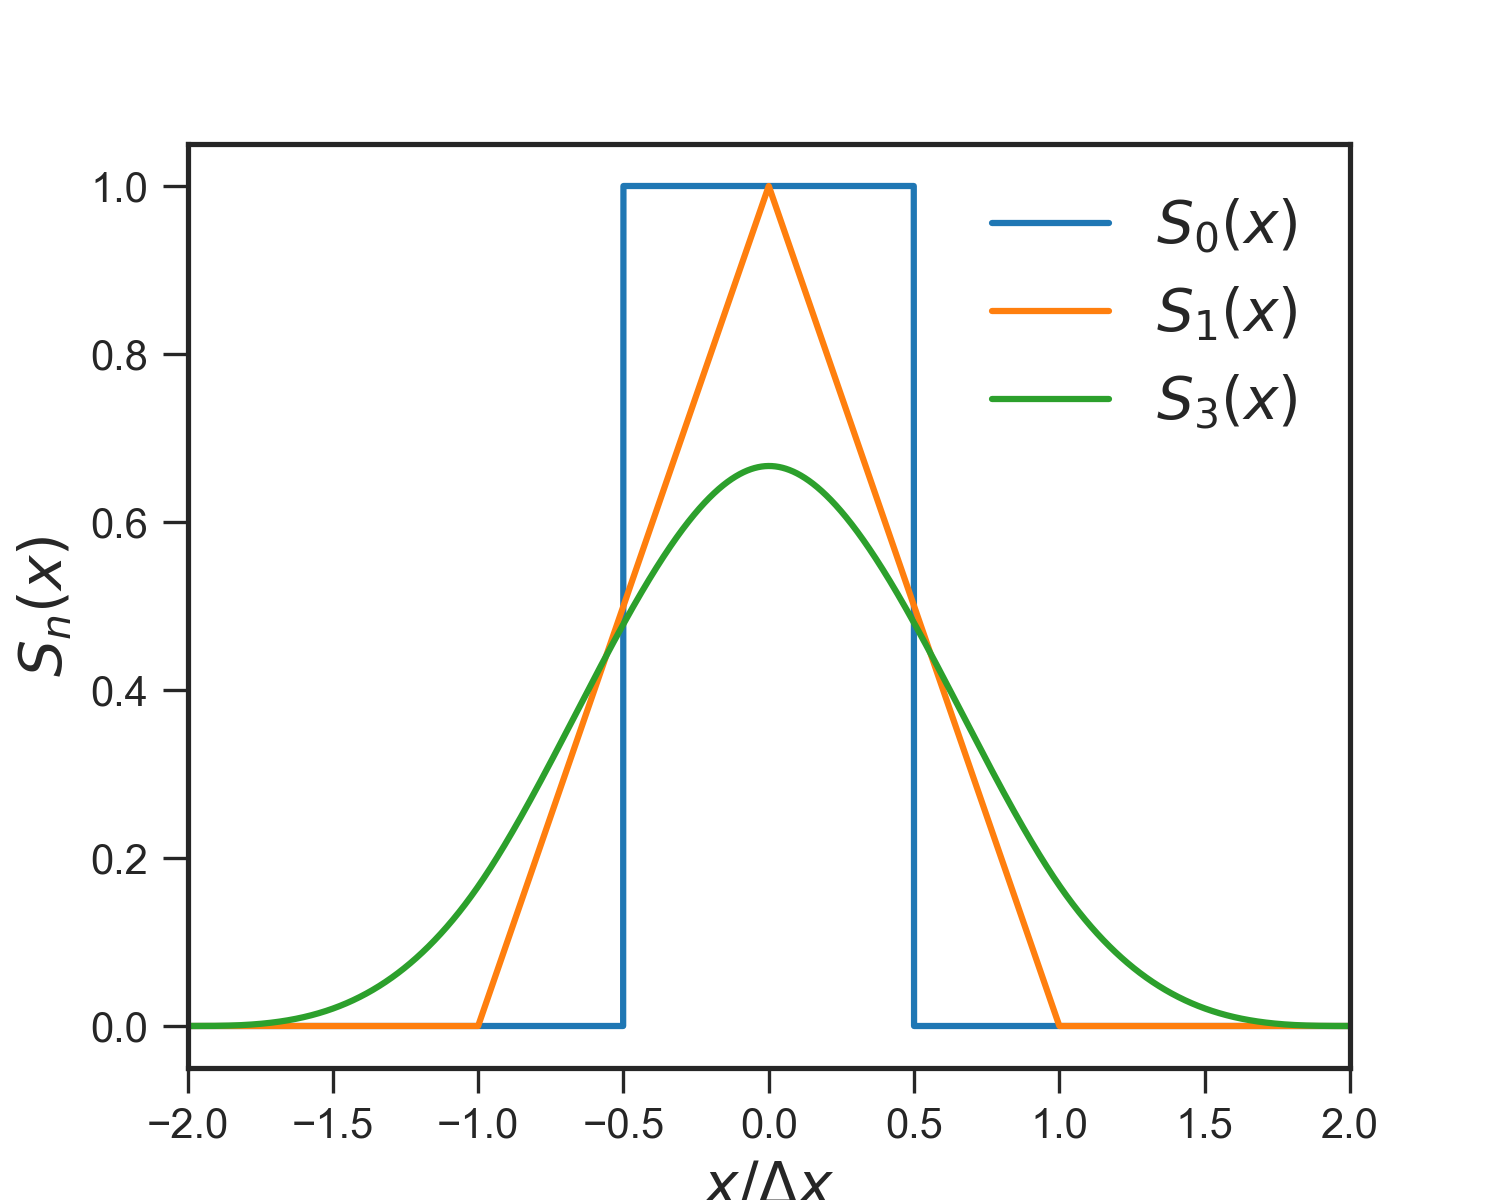
\includegraphics[width=0.6\linewidth]{planning/images/shape_functions.png}
	\caption{The top hat ($S_0(x)$), triangle ($S_1(x)$) and $3^\text{rd}$ order spline ($S_3(x)$) are plotted in 1D.}
	\label{fig:shape_factors}
\end{figure}

\begin{equation}
	S_n(x) \equiv \int_{-\infty}^\infty S_{n-1}(x')S_0(x-x') dx'
\end{equation}
the shape factors for $n \geq 2$ are commonly called n-splines. The third order spline is used in this work and weights particles over an area ($2 \Delta x$, $2 \Delta y$) and is represented in 1D by 

\begin{equation}
	b_3(x) = \begin{cases}
		\frac{1}{6}(8 - 12 \lvert \tilde{x} \rvert + 6 \tilde{x}^2 - \tilde{x}^3) & \text{if } 1 \leq \lvert \tilde{x} \rvert \leq 2 \\
		\frac{1}{6}(4 - 6 \tilde{x}^2 + 3 \tilde{x}^3) & \text{if } \lvert \tilde{x} \rvert \leq 1 \\
		0 & \text{otherwise}
	\end{cases}
\end{equation}
where $\tilde{x} \equiv x / \Delta x$ normalizes the position $x$. See \cref{fig:shape_factors} for a comparison of the three shape factors. 

\subsection{Field Solver and Particle Push}

\begin{figure}
	\centering 
	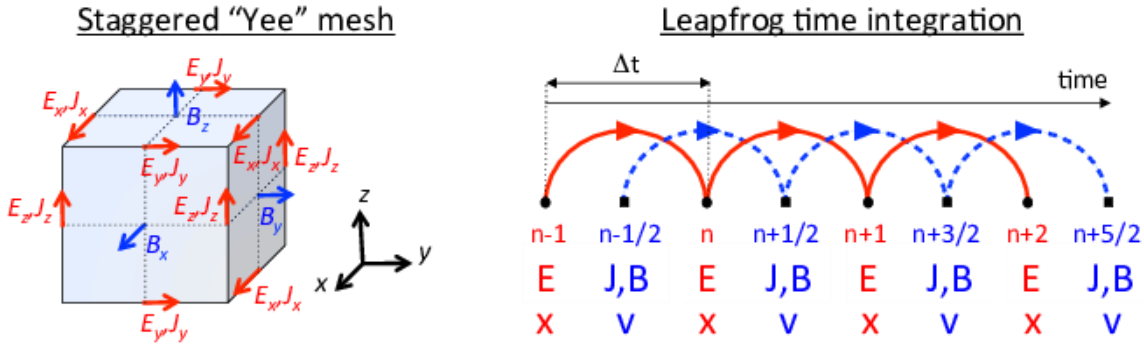
\includegraphics[width=0.8\linewidth]{planning/images/yee_grid.PNG}
	\caption{The ``Yee'' grid is depicted (left) where the electric and magnetic field components are staggered by half a cell. The fields, currents, position, and velocity make use of the staggered grid by leapfrog time integration (right). This picture was taken from the WarpX documentation}
	\label{fig:yee_grid}
\end{figure}

The PIC method is able to make efficient use of the second order accurate central difference approximation to compute derivatives. A simpler method like Euler integration is only first order accurate and will suffer in terms of accuracy. Higher order methods like 4th order Runge-Kutta have much higher computational costs in terms of operations per time step and memory consumption. The central difference scheme is accomplished by alternately calculating electric and magnetic fields, staggered by half a time step, in an approach called \emph{leapfrog integration}\cite{Birdsall_2004_PIC}. This can be seen in the right half of \cref{fig:yee_grid} where the calculations of $E$ and $J,B$ alternate in a ``leapfrog'' fashion. It turns out that this staggering also comes with some nice properties like automatically satisfying \cref{eq:gauss_magnetism}. By rearranging \cref{eq:faraday}, we can update the electric and magnetic fields through the following equations\cite{Arber_2015_PPCF}

\begin{align}
	\vec{E}^{n+\frac{1}{2}} &= \vec{E}^{n-\frac{1}{2}} + \Delta t (c^2 \nabla \times \vec{B}^n - \frac{1}{\epsilon_0} \vec{J}^n) \label{eq:E_update} \\
	\vec{B}^{n+1} &= \vec{B}^{n} - \Delta t (\nabla \times \vec{E}^{n+\frac{1}{2}}) \label{eq:B_update}
\end{align}
Given the electric and magnetic fields, we can now update the particle positions through \cref{eq:lorentz_pic}. The standard approach to update velocities and positions in a time-centered way would involve kinematics equations $v^{n+1/2} = v^{n-1/2} + a^n \Delta t$ and $x^{n+1} = x^{n} + v^{n_1/2} \Delta t$. The acceleration is both a function of $x$ and $v$ (\cref{eq:lorentz_pic}) and so cannot be calculating accurately in a time-centered way. This can be fixed through the application of the Boris rotation algorithm which removes the 

\begin{equation}
	\frac{v_{n + 1/2} - v_{n - 1/2}}{\Delta t} = \frac{q}{m}[E_n + v \times B]
\end{equation}

\subsection{EPOCH Code}

\begin{quote}
	Clearly Top-hat shape functions should never be used for laser-solid simulations.
\end{quote}

\subsection{Convergence Testing the EPOCH Code}


\section{Machine Learning}

\subsection{Simple Models}

\subsubsection{Polynomial Regression}

\subsubsection{Support Vector Regression}


\subsection{Advanced Models}

\subsubsection{Gaussian Process}

\subsection{Neural Networks}
\chapter{Particle-in-Cell Simulations of Enhanced Target Normal Sheath Acceleration} \label{ch:4}

This chapter details the work I did in conducting \gls{PIC} simulations to better understand the \gls{eTNSA} experiments at \gls{LLNL} by Nathaniel Tamminga, Joseph Snyder, and John Morrison in March of 2024. They worked at Titan which is housed in the \gls{JLF} for 5-6 weeks using their earned ``shot time'' through a LaserNet proposal. I will mostly focus on the simulation aspect of the project, but include some relevant comparisons to the experiment as needed. 

\section{Background}

\subsection{Spatially Aligned Pulses} \label{sec:spatialalign}

\begin{figure}
	\centering 
	\includegraphics[width=0.75\linewidth]{planning/images/Markey_Spectrum.PNG}
	\caption{Proton energy spectrum from 1D particle-in-cell simulations depicted for three different temporal delays (including $\Delta t = 0$) from FIG. 3 in Markey et. al. \cite{Markey_2010_PRL}.}
	\label{fig:markey_spectrum}
\end{figure}

As explained in \cref{sec:tnsa_opt}, there is generally an optimal level of pre-expansion of the target to maximize the \gls{TNSA} proton energies \cite{McKenna_2008_LaPB,Fuchs_2007_PRL}. While the pre-expansion could be due to a low contrast pulse, it could also be due to an artificially injected pre-pulse whose intensity and temporal delay are tunable. Robinson et. al. \cite{Robinson_2007_PPCF} first addresses the idea of using multiple high intensity 40 fs laser pulses with the first being one-tenth to one-quarter of the intensity of the second. They termed this novel two-stage process \emph{multiple pulse sheath acceleration}. This study actually found a reduction in peak proton energy through numerical simulations, but did find the existence of spectral peaks -- spikes in the energy spectrum as specific energies. A few years later, Markey et. al. \cite{Markey_2010_PRL} examined a similar setup experimentally, varying the temporal separation by 0.75-2.5 ps. Interestingly, they found an enhancement in the peak proton energy with a 0.75 ps separation and energy ratio of 0.4:1 between the two pulses. They conducted 1D PIC simulations shown in \cref{fig:markey_spectrum} that verify this as well.

In 2018, Ferri et. al. \cite{Ferri_2018_PoP} re-examines the same question, but uses the same intensity for both pulses. He finds that ultimately, little to no delay is optimal and as the delay gets larger, the enhancement reduces to the single pulse result. He finds the acceleration process can be affected by the second pulse for time delays as long as $\SI{0.6}{\pico \second}$ for $\SI{3}{\micro \meter}$ targets and $\SI{1}{\pico \second}$ for $\SI{6}{\micro \meter}$ targets. 

In a different approach Scott et. al. \cite{Scott_2012_APL} realized that much of the laser light that is reflected is wasted, so a mechanism to re-direct this light back into the target would be desired. They designed a target with a half-cavity foil as seen in \cref{fig:scott_half_cavity} that will take light reflected off the accelerating foil and re-reflect it back towards the accelerating foil. They find that this can increase the laser to proton energy efficiency by up to $\sim 55 \%$.

\begin{figure}
	\centering 
	\includegraphics[width=0.9\linewidth]{planning/images/scott_half_cavity.PNG}
	\caption{Schematic of the incident laser on the half-cavity target (left) in Scott et. al. \cite{Scott_2012_APL}. The radius of the cavity foil determines the delay ($\tau = 2 r/c$) between the main pulse and the post-pulse (reflected laser light of $\sim 40 \%)$ energy of the main pulse).}
	\label{fig:scott_half_cavity}
\end{figure}

%Since we're looking at a 15 micron target, I'd imagine this time would be around 2ps, but I could solve his equations to get a better estimate. This time coincides when the fastest ions have moved a distance of the order of the transverse extent of the electric sheath field.

%Explain what contrast is: peak of the laser pulse compared to the pedestal and maybe give a diagram.

\subsection{Enhanced TNSA from Ferri et. al.}

Given the results of the previous section \cite{Markey_2010_PRL,Scott_2012_APL,Ferri_2018_PoP} that use short-delay pre or post pulses, Ferri, Siminos and Fulop decided to study how spatially \emph{and} temporally aligned pulses can enhance proton acceleration. They showed that the double pulse setup can result in an almost doubling of the proton energy and five-fold enhancement in the number of protons \cite{Ferri_2019_Nat_Comm} through \gls{PIC} simulations. This phenomena, referred to as \gls{eTNSA}, is depicted in \cref{fig:ferri_dub_pulse} which shows the constructive interference of the fields at the front of the target in the center panel (e) and enhanced \gls{TNSA} fields at the target rear (f).

\begin{figure}
	\centering 
	\includegraphics[width=\linewidth]{planning/images/ferri_dub_pulse.PNG}
	\caption{Geometry of the two pulse scheme as shown in Figure 1 of Ferri et. al. (2019) \cite{Ferri_2019_Nat_Comm}. The single pulse has a total energy of 1.1J at an incidence angle of $\phi=45^\circ$ and is shown through several time snapshots (a-c). In (d-f), the double pulse is shown through those same time snapshots with energies of 0.55 J in each pulse (the 1.55 J is a typo from the original figure). Other parameters include $\tau_\text{fwhm} = \SI{38}{\femto \second}$, thickness = $\SI{3}{\micro \meter}$, material = aluminum, $w_\text{0,fwhm} = \SI{5}{\micro \meter}$, $I_0 = \SI{7e19}{\watt \per \centi \meter \squared}$.}
	\label{fig:ferri_dub_pulse}
\end{figure}
The constructive interference of the electric fields can be understood by considering the electric field of two p-polarized pulses coming in at angles of incidence $\phi$ and $-\phi$

\begin{align}
	E_{x,1} &= -E_0 \sin(\phi) \sin(k y \sin(\phi) - \omega t + k x \cos(\phi)) \\
	E_{x,2} &= -E_0 \sin(\phi) \sin(k y \sin(\phi) - \omega t - k x \cos(\phi))
\end{align}
Adding these two fields together results in 

\begin{equation}
	E_\text{double} = -2 E_0 \sin(\phi) \sin(k y \sin(\phi) - \omega t) \cos(k x \cos(\phi))
\end{equation}
which has an amplitude of $\lvert E_\text{double} \rvert = 2 E_0 \sin(\phi)$. In contrast, a single pulse with twice the energy (intensity) would only have a $\sqrt{2}$ larger electric field ($\lvert E_\text{single} \rvert = \sqrt{2} E_0 \sin(\phi)$) which explains the enhanced electric fields seen in the bottom row of \cref{fig:ferri_dub_pulse}. In an ideal situation where 100\% of the laser pulse is reflected, the angles of the two pulses do not need to be equal and opposite -- we will get a standing wave pattern from the constructive interference of the incident wave with its reflection and the same $\sqrt{2}$ field enhancement.  

Unlike the methods described in \cref{sec:spatialalign} (which see enhanced proton acceleration from a pre-expanded target), \gls{eTNSA} relies on the presence of an undisturbed target from the vacuum heating mechanism \cite{Brunel_1987_PRL} explained in \cref{sec:absorption}. Vacuum heating relies on the dominance of the electron's quiver motion in the oscillatory electric field in the x-direction, but the magnetic field (which is relevant when $a_0 \gtrsim 1$) may impart a $\vec{v} \times \vec{B}$ Lorentz force (\cref{eq:lorentz}) that negatively affects the electron acceleration in the x-direction. Brunel even assumes in his original 1987 paper \cite{Brunel_1987_PRL} that we can ignore $\vec{v} \times \vec{B}$ interactions if the laser is split into two equal and opposite angle pulses. Ferri confirms \cite{Ferri_2019_Nat_Comm}, through simulations, that the magnetic field is indeed suppressed in the double pulse case which results in hot electrons accelerated to higher energies. 

\begin{figure}
	\centering 
	\includegraphics[width=\linewidth]{planning/images/ferri_scale_energy.PNG}
	\caption{Double pulse effectiveness in terms of changing preplasma scale length (a) and total laser energy (b,c) from Ferri et. al. (2019) \cite{Ferri_2019_Nat_Comm}.}
	\label{fig:ferri_scale_energy}
\end{figure}

Furthermore, Ferri ran some simulations exploring different preplasma scale lengths $L$ at a fixed energy, and changing the total laser energy for the flat target \cite{Ferri_2019_Nat_Comm} which can be seen in \cref{fig:ferri_scale_energy}. He finds that a higher preplasma scale length generally increases the max proton energy up to a certain scale length of around $L = \SI{0.6}{\micro \meter}$. The enhancement is seen for all scale lengths, but the gap between single and double pulse diminishes for larger scale lengths. In the double pulse case, a more favorable scaling with laser energy is seen for both the hot electron temperature and maximum proton energy ($E_\text{0,tot}$ as opposed to $\sqrt{E_\text{0,tot}}$) when comparing double pulse against single. In addition, Ferri comments that, for pulses with total energy greater than 10 J, the proton layer on the rear side starts to entirely disconnect from the bulk of the target during the acceleration, causing proton energies to saturate and become lower than the expected linear scaling.

\subsection{Other eTNSA Simulations}
In 2021, \gls{eTNSA} was again demonstrated through simulations in Rahman et. al. \cite{Rahman_2021_PoP} for a mJ class laser, around 2 orders of magnitude lower energy than the setup in Ferri's work. This mJ class laser is based on the experimental facility at the Wright Patterson Air Force Base (see \cref{ch:6} for more details) which utilizes a thinner target of $\sim \SI{0.5}{\micro \meter}$. Despite the major difference in laser and target parameters, the findings are similar -- increased hot electron temperature and proton energies with double pulse compared to single pulse. However, Rahman finds that the presence of a preplasma actually \emph{reduces} the maximum proton energy. But, like Ferri et. al., the gap between single and double pulse becomes smaller in the presence of a preplasma.

In 2024, Khan and Saxena \cite{Khan_2024_NJoP} revisit the double pulse scheme but with an applied longitudinal kilo-Tesla level magnetic field. The purpose of the magnetic field is to reduce the divergence of the hot electron beam. This guides the electrons and enhances the \gls{TNSA} process to see a higher maximum cutoff energy in the proton spectrum \cite{Arefiev_2016_NJoP}. In this study, the laser was based off of the experimental set-up at \gls{RAL} with a peak intensity of $\SI{5.5e20}{\watt \per \centi \meter \squared}$ incident on a $\SI{7}{\micro \meter}$ polyethelene target. 

% Preplasma is only on front of target just like titan dub pulse sims

\subsection{Recent Experiments}

Due to multiple studies demonstrating \gls{eTNSA} \cite{Ferri_2019_Nat_Comm,Rahman_2021_PoP,Khan_2024_NJoP}, experiments are needed to validate the \gls{PIC} simulations. Morace et al. \cite{Morace_2019_Nat_Comm} showed that splitting a 270 J beam ($\SI{2.5e18}{\watt \per \centi \meter \squared}$ peak intensity) into multiple ``beamlets'' on Al foil targets enhances the proton energy spectrum. These beamlets (dependent on the incidence angle) induced critical surface density modulations that strongly improved absorption into hot electrons. 

\begin{figure}
	\centering 
	\includegraphics[width=0.75\linewidth]{planning/images/yao_exp_stacks.PNG}
	\caption{FIG. 2 from Yao et al. \cite{Yao_2024_MaRaE}. Case 0 shows electron signals from a single pulse. Case 1 shows electron signals from a double pulse with spatial separation $\SI{120}{\micro \meter}$. Case 2 shows electron signals from a double pulse with no spatial separation.}
	\label{fig:yao_exp_stacks}
\end{figure}

Yao et al. \cite{Yao_2024_MaRaE} investigated the double pulse effect by changing the transverse spatial separation between two temporally aligned pulses as shown in \cref{fig:yao_exp_stacks}. This figure shows two possible beams $\alpha$ and $\beta$ which come in at equal and opposite incidence angles with $\alpha$ angled in the $-\hat{y}$ direction. Comparing (b) and (c) shows an enhancement of the double pulse electron energy when the pulses are spatially overlapped. In (a), the electron energy is recorded along the laser beam axis in contrast to (b) and (c). This shows that most electrons are getting accelerated along the laser beam axis and the $\vec{J} \times \vec{B}$ mechanism is taking place (in contrast to vacuum heating or resonance absorption which drives electrons in the  target normal direction). In terms of the protons, case 2 (spatially aligned double pulses) shows a more collimated central small beam which is absent in case 1 (spatially offset double pulses).

\section{Titan Experiment}

The experimental setup involved one or two $50$ J or $25$ J $\sim 10^{19} \unit{\watt \per \centi \meter \squared}$ pulses arriving at a $\SI{15}{\micro \meter}$ thick gold target. The Titan laser produces $\tau_\text{FWHM} = 2$ ps pulses of wavelength $\SI{1.053}{\micro \meter}$. The beam coming from \gls{OAP}1 (\gls{OAP}2) has an incidence angle of $20^\circ$ ($42^\circ$) and spot size of $\SI{12}{\micro \meter}$ ($\SI{12}{\micro \meter}$) which can be seen in \autoref{fig:jlf_target_chamber} (the blue beam is from OAP1 and the yellow beam is from OAP2). The proton beams are recorded by three \gls{EPPS}s which are located along each beam axis and in the target normal direction.

\begin{figure}
	\centering
	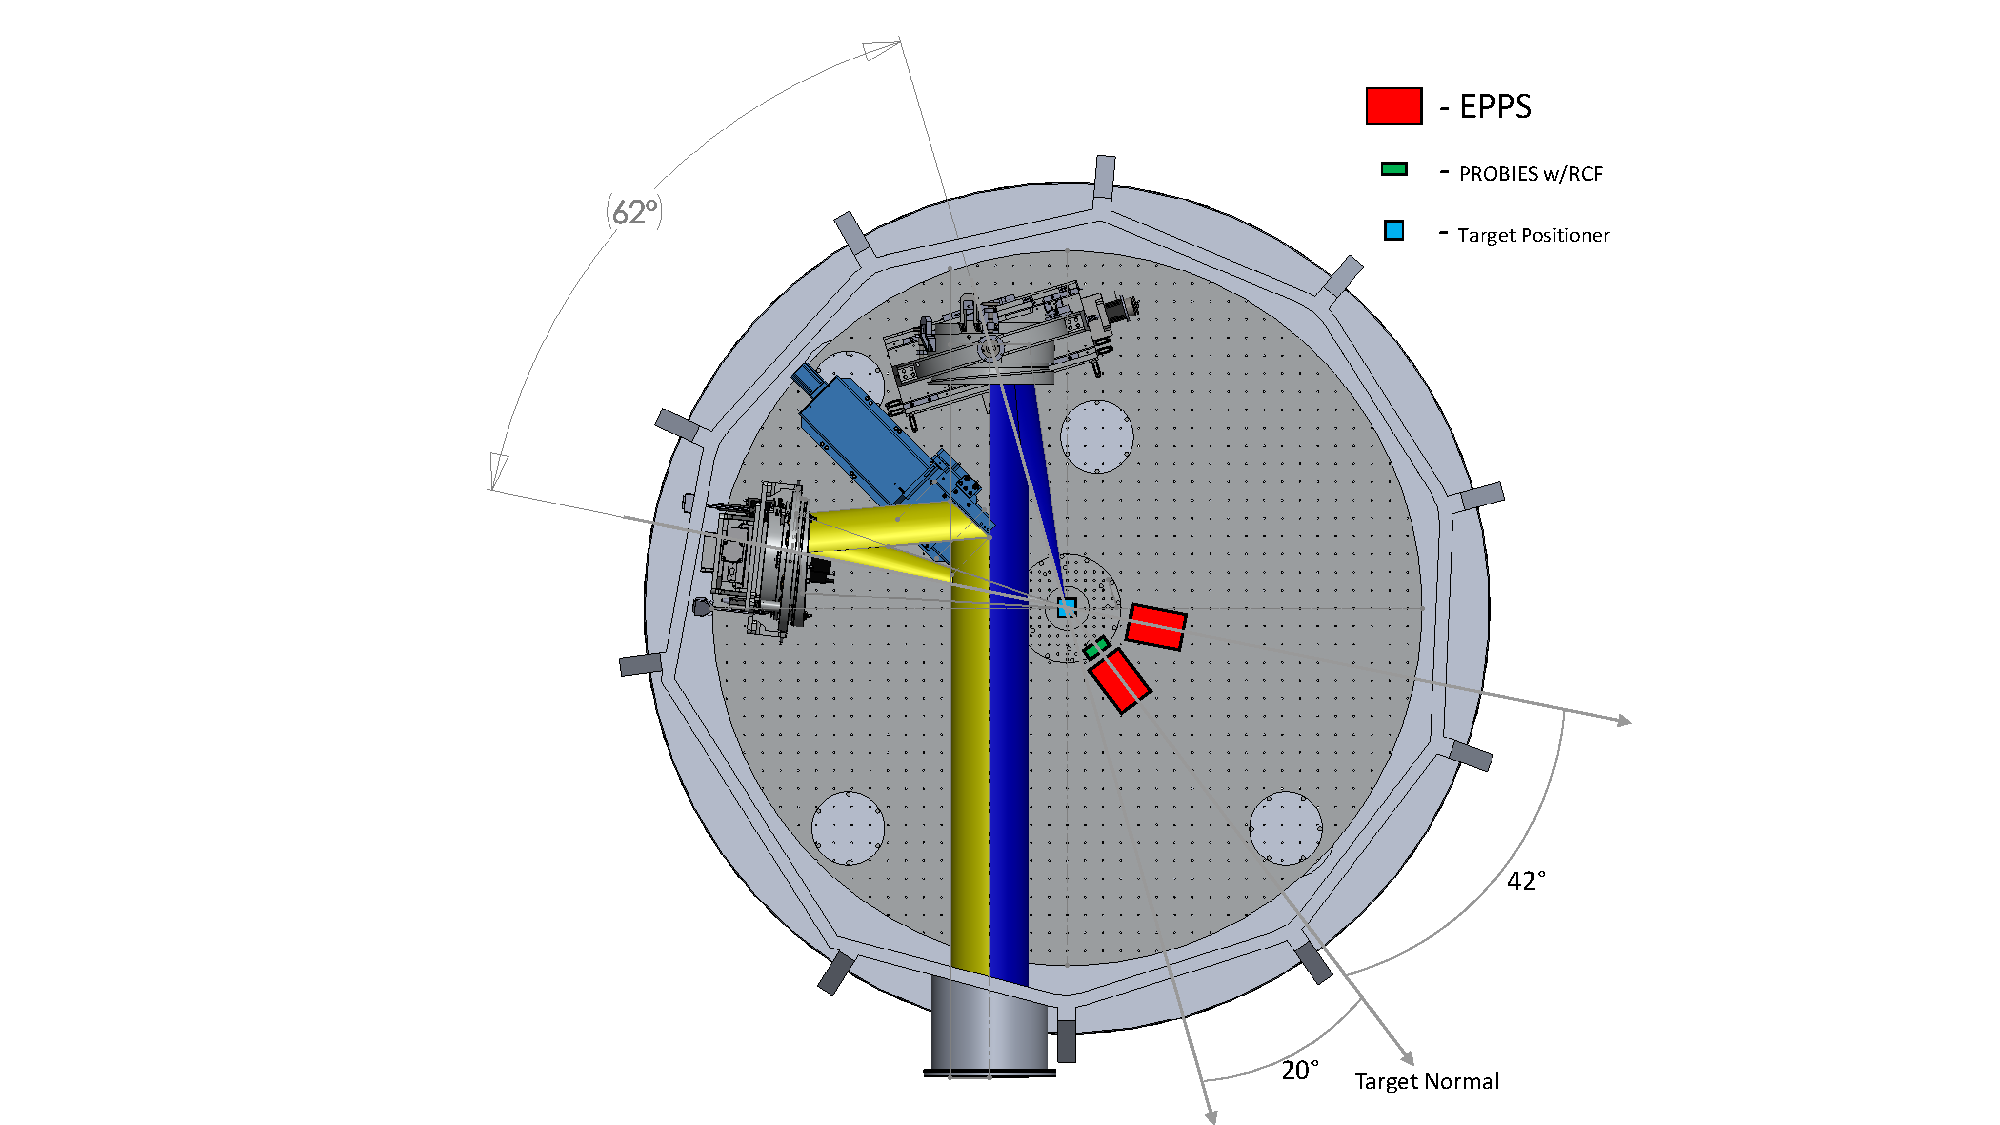
\includegraphics[width=.95\linewidth]{planning/images/titan/target_area_JLF.pdf}
	\caption{Target chamber schematic showing the split beam configuration at the LaserNet Titan experiment conducted in March of 2024. Two independent off-axis paraboloid mirrors focus each beam onto a 15~$\mu$m Au target which record proton spectra from multiple electron positron proton spectrometers.}
	\label{fig:jlf_target_chamber}
\end{figure}

\subsection{Gold Simulations}

To model this setup, we used 2D(3v) simulations using the EPOCH \gls{PIC} code (version 4.19.0). For simplicity, both pulses had a fixed spot size of $w_\text{FWHM} = \SI{12}{\micro \meter}$ to enable better comparison between the individual pulses. Using a $\SI{2e19}{\watt \per \centi \meter \squared}$ peak intensity, the single pulse would have around 65 J of energy for a sine-squared temporal profile. Accordingly, the double pulse has half the energy and intensity per pulse. We timed the pulses to arrive at the target front around 100 fs into the simulation. Even though the total pulse duration is around $2 \tau_\text{FWHM} = \SI{4}{\pico \second}$, we only run the simulations to 2.2 ps which is more than sufficient to see the highest energy protons produced. Note that there are two single pulse cases, but the figures below choose \gls{OAP}2 ($41^\circ$) due to higher sheath fields, electron energies, and proton energies observed throughout the simulations as can be seen in \autoref{tab:gold_sims}.

The $\SI{15}{\micro \meter}$ thick target had a length of $\SI{36}{\micro \meter}$ which can be seen in FIGURE rotated at a $45^\circ$ angle. The gold target had an initial number density $n_0 = \SI{5.9e28}{\per \meter \cubed}$ and a $\SI{0.5}{\micro \meter}$ layer of protons (of the same density) was added to the rear side to enhance the \gls{TNSA} effect.  The gold was initially neutral and allowed to freely ionize through EPOCH's field ionization routine (typically reaching $Z^* = 20$ or $Z^* = 30$ after 1 to 2 ps respectively). No recombination model was used. We employed a ($-\SI{28}{\micro \meter}$, $\SI{42}{\micro \meter}$) square simulation box with $\Delta x = \SI{13.33}{\nano \meter}$ cells and 25 (125) \gls{PPC} for gold (protons).

\begin{figure}
	\centering
	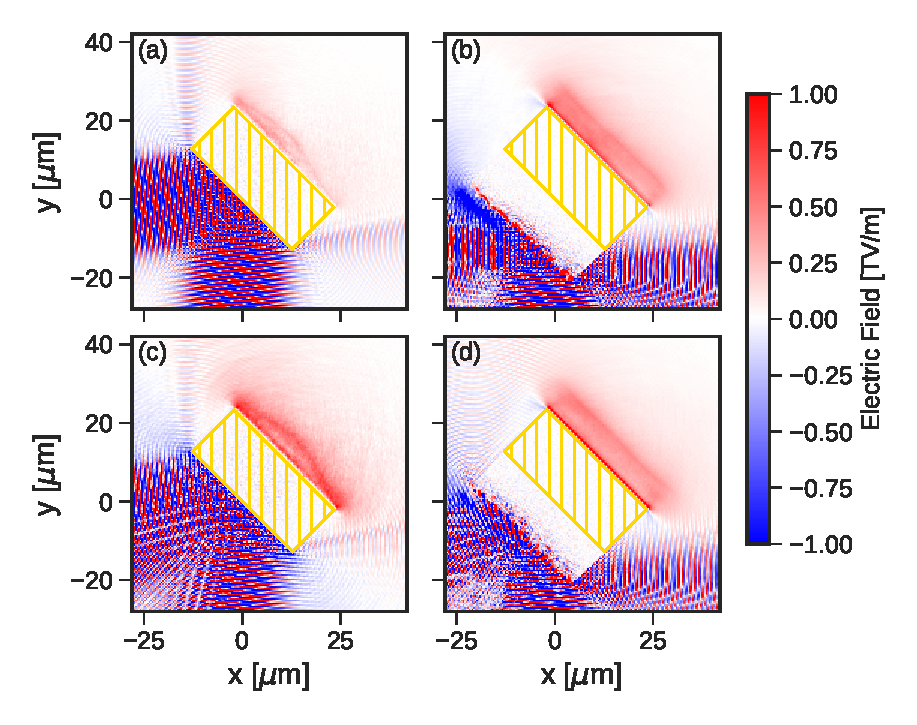
\includegraphics[width=0.9\linewidth]{planning/images/titan/efield_800fs.eps}
	\caption{Electric field in the target normal direction at simulation time of 800 fs for the (a) flat single $41^\circ$ pulse, (b) expanded single $41^\circ$ pulse, (c) flat double pulse, (d) expanded double pulse (on gold 65 J). The hatched gold rectangle is overlaid for a visual of the size of the initial, unperturbed target.}
	\label{fig:efield_800fs}
\end{figure}

From the results of Ferri et al. \cite{Ferri_2019_Nat_Comm}, we would expect the constructive interference of the pulses in front of the target to enhance the electric fields on the back side of the target. This is exactly what we see in \autoref{fig:efield_800fs}(a, c) which is an electric field snapshot 800 fs into the simulation when sheath fields are clearly developed. Furthermore, the proton energy enhancement can be seen in \autoref{fig:sim_protons_angular}(a, c) in both the maximum energy and total amount of high energy protons. This plot determines the angular direction of the protons from using the $\texttt{atan2}$ with the y and x momentum components and bins the protons by angle and energy.

\begin{figure}
	\centering
	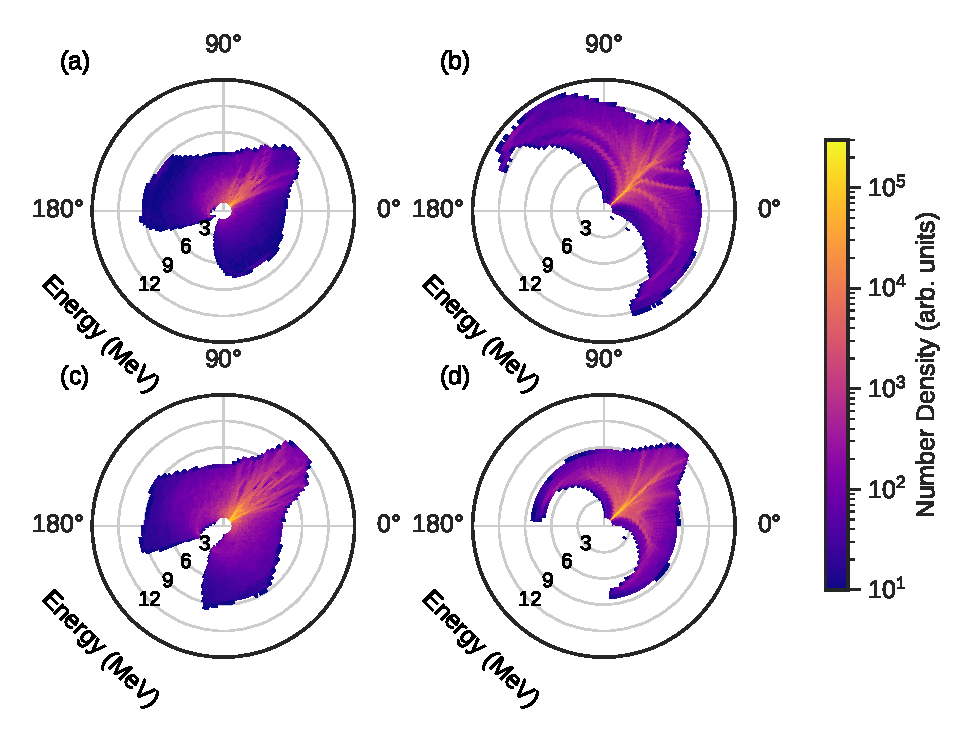
\includegraphics[width=0.9\linewidth]{planning/images/titan/proton_angular_density_2100fs.eps}
	\caption{Proton distribution as a function of angle $\phi = \tan^{-1}(p_y, p_x)$ and energy at simulation time of 2100 fs for the (a) flat single $41^\circ$ pulse, (b) expanded single $41^\circ$ pulse, (c) flat double pulse, (d) expanded double pulse (gold 65 J). Only protons with energy greater than 1 MeV are plotted. }
	\label{fig:sim_protons_angular}
\end{figure}

Since the presence of a pre-plasma is known to greatly affect the proton energy spectrum, we performed two additional simulations where an exponential scale $L_s = \SI{2}{\micro \meter}$ pre-plasma was placed in front of the target of the form: 

\begin{equation}
	n(r) = n_0^* \exp(-r / L_s) \label{eq:exponential_scale_pp}
\end{equation}
where $n_0^* = \SI{5.2e28}{\per \meter \cubed}$ is chosen to be lower than $n_0$ to preserve the same number of particles. This extends from $r=0$ (the target front) to $r = r_\text{cut} = \SI{15.7}{\micro \meter}$ in front of the target which corresponds to the location where the gold density would be $n_c / 50$. Here, $n_c \approx 10^{27} \unit{\per \meter \cubed}$ is the critical density (from \autoref{eq:criticaldensity}). This pre-plasma will make the critical density surface at which the laser primarily delivers energy into the target around $r = \SI{8}{\micro \meter}$ in front of the target which can be seen in the electric fields of \autoref{fig:efield_800fs}(b, d). From this figure, the electric field enhancement on the rear side of the target is not clear, but the proton energy distribution from \autoref{fig:sim_protons_angular}(b, d) show that the double pulse clearly focuses the proton beam to a narrower angular spread and reduces filamentation. Additionally, the number of protons along the target normal direction is higher in the double pulse case as can be seen from the colorbar. 

\begin{figure}
	\centering
	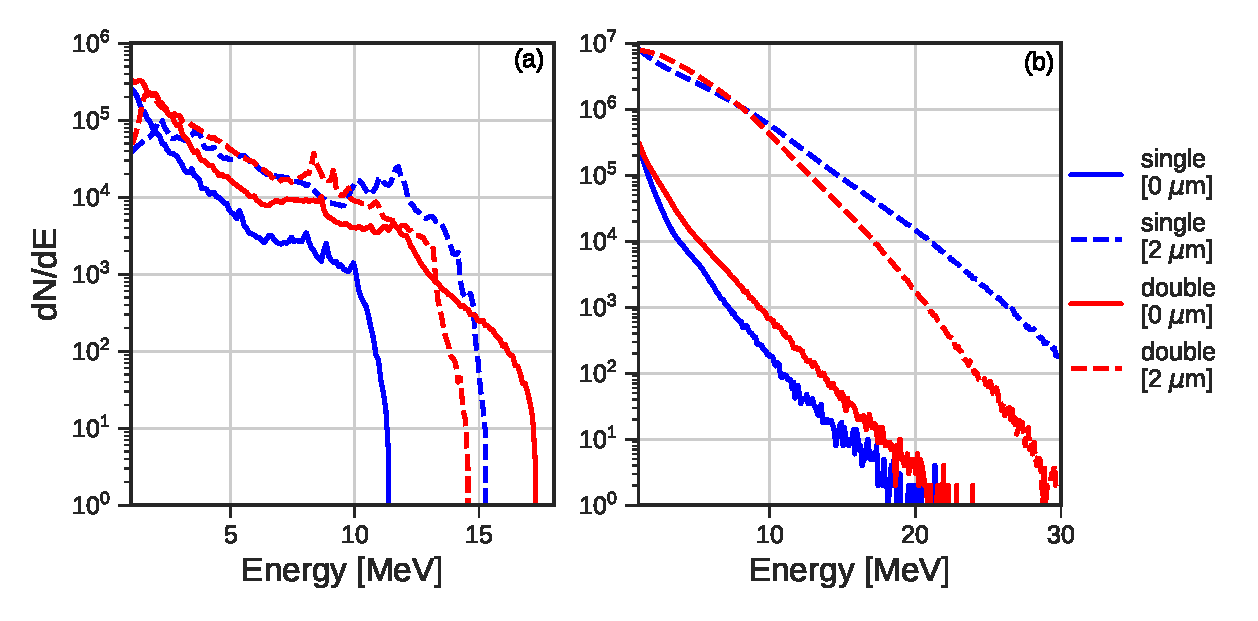
\includegraphics[width=0.9\linewidth]{planning/images/titan/spectrum_2100fs.eps}
	\caption{Spectrum at 2100 fs for (a) protons and (b) electrons (gold 65 J). Particles that have left the simulation before 2100 fs are included in the spectrum from their energy at the time of crossing the boundary.}
	\label{fig:sim_spectrum}
\end{figure}

To make these trends clear, the proton energy spectra at 2.1 ps were plotted in \autoref{fig:sim_spectrum} for each of the single an double pulses with and without the $\SI{2}{\micro \meter}$ pre-plasma. We can clearly see (a) that the proton energy spectrum is enhanced for the double pulse without pre-plasma, but this is not so clear for the case with pre-plasma. Furthermore, the electron energy spectra (b) shows a clear enhancement in electron energy in the presence of pre-plasma. 

\begin{figure}
	\centering
	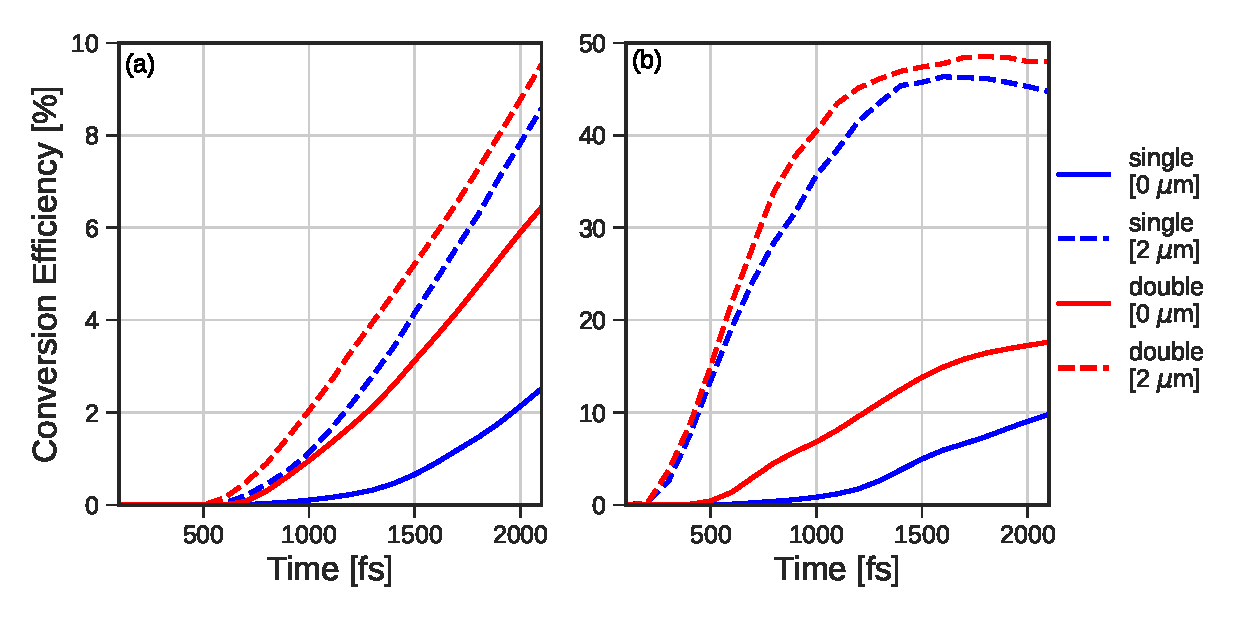
\includegraphics[width=0.9\linewidth]{planning/images/titan/conversion_efficiency.eps}
	\caption{Conversion Efficiency of Laser Energy into greater than 1 MeV (a) protons and (b) electrons for 65 J simulations on gold.}
	\label{fig:sim_conv_eff}
\end{figure}

Another metric would be the overall conversion efficiency of laser energy into high energy ($> 1 $ MeV) electrons or protons which is shown in \autoref{fig:sim_conv_eff}. This is computed by dividing the energy in high energy protons or electrons by the total laser energy that entered the simulation at that point in time. Here it becomes more clear that there is a proton and electron energy enhancement in the double pulse case for both flat and pre-expanded targets. Although, it bears mentioning that the enhancement is much smaller in the presence of a pre-plasma. 

\renewcommand{\arraystretch}{1.15}
\setlength{\tabcolsep}{0.5em}
\begin{table}
	\centering
	\begin{tabular}{|c|c|c|c|c|p{1.4cm}|c|p{1.4cm}|c|}
		\hline
		\hline
		\textbf{Pulse} & $\pmb{\theta}_i$ & $\mathbf{I}_0$ [$\frac{\text{W}}{\text{cm}^2}$]  & $\mathbf{E}_\text{laser}$ [J] & $\mathbf{L}_p$ [$\mu$m] & $\mathbf{KE}_\text{p,max}$\newline [MeV] & $\pmb{\eta}_\text{p}$ [\%] & $\mathbf{KE}_\text{e,max}$\newline [MeV]& $\pmb{\eta}_{\text{e}}$ [\%] \\
		\hline 
		Single & $20^\circ$ & $2 \times 10^{19}$ & 65 & 0 & 8.5 & 0.5 & 29.8 & 2.0 \\
		\hline
		Single & $41^\circ$ & $2 \times 10^{19}$ & 65 & 0 & 11.35 & 2.5 & 33.48 & 9.8 \\
		Double & $20^\circ, 41^\circ$ & $1 \times 10^{19}$ & 65 & 0 & 17.2 & 6.4 & 27.2 & 17.6 \\
		Single & $41^\circ$ & $2 \times 10^{19}$ & 65 & 2 & 15.4 & 8.6 & 37.6 & 44.7 \\
		Double & $20^\circ, 41^\circ$ & $1 \times 10^{19}$ & 65 & 2 & 14.6 & 9.5 & 31.4 & 48.0 \\
		\hline 
		Single & $41^\circ$ & $1 \times 10^{19}$ & 32.5 & 0 & 9.0 & 1.5 & 14.6 & 5.3 \\
		Double & $20^\circ, 41^\circ$ & $5 \times 10^{18}$ & 32.5 & 0 & 13.9 & 4.4 & 21.3 & 11.4 \\
		Single & $41^\circ$ & $5 \times 10^{18}$ & 16.3 & 0 & 6.4 & 0.6 & 9.7 & 2.0 \\
		Double & $20^\circ, 41^\circ$ & $2.5 \times 10^{18}$ & 16.3 & 0 & 10.6 & 2.5 & 10.1 & 6.0 \\
		\hline
		\hline
	\end{tabular}
	\caption{Summary of Gold Simulations.}
	\label{tab:gold_sims}
\end{table}

\subsection{Comparison to Experiment}

\section{Discussion}


\chapter{Machine Learning Methods Applied to Synthetic Ion Acceleration Data} \label{ch:5}

This chapter details the work I did developing and investigating a synthetic dataset based on a model by Fuchs \cite{Fuchs_2005_Nat}.

\section{Modified Fuchs et. al. Model}

In this section, I will describe the model from which we generated the synthetic datasets \cite{Desai_2024_CPP,Desai_2024_arX}. First, the expansion of a plasma into a vacuum \cite{Mora_2003_PRL} is used to determine the maximum proton energy and the number of accelerated protons per unit energy $\frac{dN}{dE}$. Following Fuchs \cite{Fuchs_2005_Nat}, we introduce define the acceleration time in proportion to the pulse duration of the laser and adopt a scaling (e.g. \cref{eq:wilks}) to relate hot electron temperature to the ponderomotive potential. This, in combination with other empirical estimates, allows calculating a proton energy spectrum from up to 7 parameters: main pulse intensity, contrast, wavelength, pulse duration, target thickness, target focal position, and laser spot size.

\subsection{Plasma Expansion into a Vacuum}

This model was developed by Mora \cite{Mora_2003_PRL} in 2003 who built off of earlier efforts \cite{Crow_1975_JPP,Kishimoto_1983_PoF} in examining an isothermal expansion model. The model begins with the assumption that ions are contained in the semi-infinite interval $n_i = n_{i0}$ for $x < 0$ and no ions initially in the vacuum region for $x > 0$. The electrons are distributed according to the boltzmann relation given by \cref{eq:boltzmann} where $n_{e0} = n_e(x = -\infty)$ is the electron density in the unperturbed plasma. Through this relation, $\phi(-\infty) = 0$. The initial electron density is related to the ion density $n_{e0} = Z n_{i0}$ where $Z$ is the ion charge number for a fully ionized plasma. The potential also satisfies the Poisson equation \cref{eq:poisson} where $\rho/m = - e (n_e - Z n_i)$ is the mass density of the electrons. The solution of \cref{eq:poisson} at $t=0$ is found by integration \cite{Crow_1975_JPP} (where $E \equiv -\frac{d\phi}{dx}$) as 

\begin{equation}
	\frac{1}{2} \epsilon_0 E^2 = n_{e0} k_B T_e
	\begin{cases}
		\exp(\frac{e \phi}{k_B T_e} - 1 - \frac{e \phi}{k_B T_e}) & \mbox{if x < 0} \\
		\exp(\frac{e \phi}{k_B T_e}) & \mbox{if x > 0} \label{eq:crow_field}
	\end{cases}
\end{equation} 
From enforcing continuity of \cref{eq:crow_field} at $x=0$ (the location of the ion front initially) we determine $\phi = -k_B T_e / e$ to arrive at  

\begin{equation}
	E_{front,0} = \sqrt{\frac{2}{\exp(1)}} E_0
\end{equation}
where $E_0 \equiv \sqrt{n_{e0} k_B T_e / \epsilon_0}$. To get an estimate of the electric field at the ion front when $t > 0$ we need to consider what the characteristic time scale for ion motion is: the plasma ion frequency $\omega_{p,i}$

\begin{equation}
	\omega_{p,i} \equiv \sqrt{\frac{Z n_{e0} e^2}{m_i \epsilon_0}}	\label{eq:omegapi}
\end{equation} 
which is analogous to \cref{eq:omegape} So, in relation to the time-scale of plasma ion oscillations, a long time would refer to $\omega_{p,i} t \gg 1$. The ion fluid sound speed $c_s$ is given by 

\begin{equation}
	c_s = \sqrt{\frac{Z k_B T_e}{m_i}} \label{eq:soundspeed}
\end{equation}
and which is very similar to \cref{eq:vthermal} Using the definition of the debye length (\cref{eq:debye}) and sound speed $c_s$ we can re-express \cref{eq:omegapi} as 

\begin{equation}
	\omega_{p,i} t = \sqrt{\frac{Z k_B T_e}{m_i}} \sqrt{\frac{n_{e0} e^2}{\epsilon_0 k_B T_e}} t = (c_s t) (\lambda_{D0})
\end{equation}
where $\lambda_{D0}$ is the initial Debye length and $c_s$ is the ion sound speed. As we know from \cref{ch:2}, when $\lambda_D$ is smaller than the characteristic length scale of a system, the quasi-neutrality condition for a plasma is satisfied. In this case, the length scale would be $c_s t$ and we can show that asserting the condition $\omega_{p,i} t > 1$ is equivalent to $\lambda_D < c_s t$. We can continue by incorporating equations of continuity and the Lorentz force (\cref{eq:lorentz}) which can be expressed as 

\begin{subequations}
	\begin{align}
		\frac{\partial n_i}{\partial t} + v_i \frac{\partial n_i}{\partial x} &= - n_i \frac{\partial v_i}{\partial x} \label{eq:continuity} \\
		\frac{\partial v_i}{\partial t} + v_i \frac{\partial v_i}{\partial x} &= -\frac{Z e}{m_i} \frac{\partial V}{\partial x} \label{eq:lorentz_mora}
	\end{align}
\end{subequations}
This set of fluid equations can be solved numerically with the initial conditions for $n_i$, $E$, and $v_i = 0$, but it is more instructive to consider a ``self-similar solution'' that describes the ions moving with speed 
\begin{equation}
	v_i = c_s + x/t \label{eq:selfsimilarvelocity}
\end{equation}
for $x + c_s t > 0$. It is self-similar in the sense that the specific length and time scales are not important, only their ratio $x/t$. In this self-similar region, quasi-neutrality is maintained and the expanding electron density can be expressed as

\begin{equation}
	n_e = Z n_i = n_{e 0} \exp(-\frac{x}{c_s t} - 1) \label{eq:selfsimilardensity}
\end{equation} 
By combining \cref{eq:continuity,eq:lorentz_mora,eq:selfsimilarvelocity,eq:selfsimilardensity}, we can arrive at a solution for the self-similar electric field in this quasi-neutral region

\begin{equation}
	E_{SS} = \frac{m_i c_s}{Z e t} = \frac{k_B T_e}{e c_s t} = \frac{E_0}{\omega_{p,i} t} \label{eq:selfsimilarefield}
\end{equation}
Physically, we can interpret this as a sheet of positive charge $\sigma = \epsilon_0 E_{SS}$ at $x = - c_s t$ and a sheet of negative charge $-\sigma$ at the plasma edge. The location of this plasma edge (i.e. the location of the ion front) can be roughly obtained by equating the local Debye length $\lambda_D = \lambda_{D0} \sqrt{n_{e0}/n_e}$ to the scale length $c_s t$.

\begin{equation}
	x_{i, front} = c_s t [2 \ln(\omega_{p,i} t) - 1] \label{eq:mora_xfront}
\end{equation} 
and the ion velocity at the front can also be obtained 

\begin{equation}
	v_{i, front} = 2 c_s \ln(\omega_{p,i} t)
\end{equation}
The ion velocity can plug back into \cref{eq:lorentz_mora} to find out that $E_\text{front,SS} = 2 E_{SS}$. Mora found an approximate solution to $E_{front}$ that matches $E_\text{front,0}$ and $E_\text{front,SS}$ in their respective cases ($t = 0$ and $\omega_{p,i} t \gg 1$) as 

\begin{equation}
	E_{front} \simeq \frac{2 E_0}{\sqrt{2 \exp(1) + (\omega_{p,i} t)^2}}
\end{equation}

\begin{figure}
	\centering 
	\subfloat{
		\label{fig:fig1_mora}
		\includegraphics[width=0.5\linewidth]{planning/images/fig1_mora.PNG}
	}
	\subfloat{
		\label{fig:fig2_mora}
		\includegraphics[width=0.5\linewidth]{planning/images/fig2_mora.PNG}
	}
	\caption{The net charge density (left) as a function of position $x / c_s t$ and normalized electric field $E/E_0$ (right) for $\omega_{pi} t = 50$ taken from Fig 1 and 2 in Mora's Paper \cite{Mora_2003_PRL}. On the right, the self-similar electric field from \cref{eq:selfsimilarefield} is plotted with a dashed line.}
\end{figure}
This formula not only reaches the correct values in the limiting cases, but also effectively interpolates in the intermediary regions (i.e. $\omega_{p,i} t \sim 1$) when compared to a numerical code that solves \cref{eq:continuity,eq:lorentz_mora} without assuming a self-similar solution. In \cref{fig:fig1_mora}, we see the net charge density at some time $\omega_{pi} t = 50$ after the start of a 1D plasma expansion simulation. We can identify the $-2\sigma$ with the fastest expanding electrons and the $+\sigma$ region next to it as the positive ions getting pulled along. In \cref{fig:fig2_mora}, we can see the electric field between these two charged regions peaks $\simeq 2 E_{ss}$. Then, using this formula with $\cref{eq:lorentz_mora}$, we can determine the ion front velocity as 

\begin{equation}
	v_{i,front} = 2 c_s \ln(\tau + \sqrt{\tau^2 + 1})	
\end{equation}
where we've defined a normalized acceleration time $\tau \equiv \omega_{p,i} t / \sqrt{2 \exp(1)}$. Additionally, in the limit $\omega_{p,i} t \gg 1$, \cref{eq:mora_xfront} becomes

\begin{equation}
	x_{i, front} \simeq c_s t [2 \ln(\omega_{p,i} t) + \ln(2) - 3] \label{eq:mora_xfront_simple}
\end{equation}
The per-ion kinetic energy can now be calculated as

\begin{align}
	\mathcal{E} \equiv \frac{1}{2} m_i v_{i,front}^2 &= 2 m_i c_s^2 \ln(\tau + \sqrt{\tau^2 + 1})^2  \nonumber\\
	&= 2 Z k_B T_{e} \ln(\tau + \sqrt{\tau^2 + 1})^2 \label{eq:mora_maxE}
\end{align}
Using \cref{eq:selfsimilardensity}, we can determine the number of accelerated ions between $x = -c_s t$ and $x = x$ as

\begin{equation}
	N_i \equiv \int_{-c_s t}^{x} n_i(x') dx' = n_{i0} c_s t [1 - \exp(-\frac{x}{c_s t} - 1)]
\end{equation}
and using \cref{eq:selfsimilarvelocity}, we can show that this is equivalent to 

\begin{equation}
	N_i(x) = n_{i0} c_s t [1 - \exp(-\sqrt{\frac{2 \mathcal{E}}{\mathcal{E}_0}})] \label{eq:numprotons}
\end{equation}
where $\mathcal{E}_0 \equiv Z k_B T_e$. Now that the number of ions is expressed in terms of the energy $\mathcal{E}$, we can determine the number of accelerated ions per unit energy (per unit surface) as 

\begin{equation}
	\frac{d N}{d \mathcal{E}} = \frac{n_{i0} c_s t}{\sqrt{2 \mathcal{E} \mathcal{E}_0}} \exp(-\sqrt{\frac{2 \mathcal{E}}{\mathcal{E}_0}}) \label{eq:dNdE}
\end{equation}
	
\subsection{Modified Fuchs Model} \label{sec:fuchsv1}

When $\tau \rightarrow \infty$, \cref{eq:mora_maxE} diverges to $\infty$. This is an inherent limitation of the isothermal fluid model, and different models are able to avoid this issue \cite{Mora_2005_PRE,Passoni_2010_NJoP,Schreiber_2006_PRL}. However, a simple fix to this model involves assuming that this acceleration time is finite and proportional to the pulse duration. Physically, it makes sense that the protons are only getting accelerated on the timescale of  laser-target interactions. This is the approach taken by Fuchs \cite{Fuchs_2005_Nat} and he expresses \cref{eq:mora_maxE} as 

\begin{equation}
	E_\text{max} = 2 k_B T_h [\ln(t_p + \sqrt{t_p^2 + 1})]^2 \label{eq:fuchs_maxE}
\end{equation}
where $\tau \equiv \omega_{p,i} t_\text{acc} / \sqrt{2 \exp(1)}$ just like the Mora model. We've also set $Z=1$ to signify that we are looking for hydrogen ions (i.e. protons) The crucial difference is that we express the acceleration time as 

\begin{equation}
	t_\text{acc} \approx 1.3 \tau_\text{FWHM} \label{eq:fuchs_multiplier}
\end{equation}
One can assume that the absorption fraction of hot electrons $\eta$ (with respect to the total laser energy $E_L$) is given by $\eta_e = 1.2 \times 10^{-15} I^{0.74} \text{ W cm}^{-2}$ with a maximum of 0.5, determined from empirical scalings (e.g. see fig. 3 from Key \cite{Key_1998_PoP}). Additionally, the average energy of the hot electrons is set by the Wilks scaling \cref{eq:wilks}. Putting this together, 

\begin{equation}
	N_e = \eta_e \frac{E_L}{T_h}
\end{equation}
would be the total number of hot electrons accelerated into the target. These electrons spread out in a roughly cylindrical volume of area $S_\text{sheath}$ and length $c \tau{fwhm}$ where the circular sheath cross section can be estimated by $S_\text{sheath} = \pi (r_0 + d \tan(\theta))^2$. Here, $r_0 = w(x) \frac{\sqrt{2 \ln(2)}}{2}$ is half of the (spatial) full width at half maximum of the intensity distribution at position $x$. The effective radius of the sheath has an additional factor of $d \tan(\theta)$ where $d$ is the initial target thickness and $\theta$ is the half-angle divergence of the hot electron within the target (taken as $\theta = 25^\circ$). As a result, the hot electron number density can be expressed as 
	
\begin{equation}
	n_{e0} = \frac{N_e}{c \tau_\text{fwhm} S_\text{sheath}}
\end{equation}
With an estimate of the hot electron density, the proton spectrum can now be computed from \cref{eq:dNdE} as 

\begin{equation}
	\frac{dN}{dE} = N_0 \frac{\exp(-\sqrt{2 E/k_B T_h})}{\sqrt{2 E k_B T_h}} \label{eq:dNdE_Fuchs}
\end{equation}
where $N_0 \equiv n_{e0} c_s t_\text{acc} S_\text{sheath}$ is defined for convenience. Using a dimensionless scale for energy $\varepsilon \equiv \sqrt{2 E / k_B T_h}$, we can calculate the number of protons and total energy in protons through integrating \cref{eq:dNdE_Fuchs}

\begin{align}
	N &= N_0 (\exp(-\varepsilon_\text{min}) - \exp(-\varepsilon_\text{max})) \label{eq:fuchs_N} \\
	E_\text{tot} &= N_0 \frac{k_B T_h}{2}[\exp(-\varepsilon_\text{min})(2 + \varepsilon_\text{min}(2 + \varepsilon_\text{min})) - \exp(-\varepsilon_\text{max})(2 + \varepsilon_\text{max}(2 + \varepsilon_\text{max}))] \label{eq:fuchs_totE}
\end{align}
where $\varepsilon_\text{min} = \sqrt{2 E_\text{min} / k_B T_h}$ defines a minimum energy cutoff ($\varepsilon_\text{max}$ is analogous and chosen by \cref{eq:fuchs_maxE}). Furthermore, we can calculate the average proton energy by dividing \cref{eq:fuchs_N} from \cref{eq:fuchs_totE}

\begin{equation}
	E_\text{avg} \equiv \frac{E_\text{tot}}{N}
\end{equation}
The combination of \cref{eq:fuchs_maxE,eq:dNdE_Fuchs} have been tested across many of the early TNSA experiments of the early 2000s for a wide range of laser intensities and pulse durations with good accuracy (see fig. 4 from Fuchs \cite{Fuchs_2005_Nat}).

\subsection{Further Model Modifications} \label{sec:fuchsv2}
When restricted to a particular laser system, the wavelength, pulse duration, and spot size are fixed. Considering the model in \cref{sec:fuchsv1}, only three adjustable parameters would be of interest -- target thickness $d$, peak intensity $I_0$ and target focal position $x$. To introduce complexity into our model, we wanted to consider the effect that a pre-expanded target would have on the proton acceleration. The pre-expansion may enhance the hot electron generation, but expansion on the rear side of the target would reduce the effectiveness of the TNSA process. We incorporate this effect by allowing the laser to have a finite contrast $\kappa$ which relates the intensity of the main laser pulse $I_0$ to the intensity of a secondary laser pulse $I_\text{pre}$ as $I_\text{pre} = \kappa$. This pre-pulse is treated as a spike in intensity that occurs $t_0$ before the arrival of the main pulse. The pre-expanded target would have a new effective thickness given by 

\begin{equation}
	d_\text{eff} = d + 2 c_s t_0 \label{eq:d_eff}
\end{equation}
where $c_s$ is the ion sound speed from \cref{eq:soundspeed} in which the target is expanding outwards from both sides. Here $T_e$ is the temperature due to the pre-pulse and can be calculated by assuming that $T_e \propto I$ and that an intensity of $10^{12} \text{ W cm}^{-2}$ produces electron temperatures of $T_\text{pre,0} = 50$ eV. Since $n_e$ decreases as $d$ gets larger and $\omega_{p,i} \propto \sqrt{n_e}$, \cref{eq:fuchs_maxE} is inversely proportional to the target thickness. So, a larger prepulse with a longer time to expand $t_0$ will see a higher effective target thickness. Furthermore, when the target is off focus, the effective pre-pulse intensity on target is less which results in less expansion.

In addition, some of the main pulse energy can be depleted by traveling through the underdense region of this new pre-expanded target. These effects will be referred to as \emph{pump depletion} and are inspired by arguments from Decker \cite{Decker_1996_PoP}. Decker describes pump depletion as an ``etching'' process where traveling through the plasma causes wavefront edge to recede at a speed given by the ``etching velocity'' 

\begin{figure}
	\centering 
	\includegraphics[width=0.6\linewidth]{planning/images/density_profile.png}
	\caption{The electron density profile of the pre-expanded target is depicted for various times $t_0$. In this figure, $n(0) \equiv n_\text{max}$. Taken from Desai et al. \cite{Desai_2024_arX} where $z$ was used as the distance along the laser axis instead of $x$ as done in this work. }
	\label{fig:density_profile}
\end{figure}
\begin{equation}
	v_\text{etch} = (\omega_{p,e}/\omega)^2 c \label{eq:vetch}
\end{equation}
Note that this speed continuously changes throughout the exponential-scale electron density which falls off like $n \sim \exp(-x/c_s t_0)$ on both sides of the target (see \cref{fig:density_profile} for a visual). Due to conservation of particle number, if the target expands, the maximum density $n\text{max}$ will also lower and is given by $n_\text{max} = \frac{n_{e0} d}{d_\text{eff}}$. We can integrate $v_\text{etch}$ with respect to time, but it is more convenient in terms of the position since we know the range over which the under-dense plasma exists. The plasma edge $x_f$ is given by \cref{eq:mora_xfront_simple} and we will integrate up to the location of the critical density $x_0 = c_s t_0 (\ln(n_\text{max}) - \ln(n_c))$. Utilizing the change of variables $dx = c dt$ (due to the pulse traveling at the speed of light $c$), the ``etching distance'' can be calculated as \cite{Desai_2024_arX} 

\begin{equation}
	L_\text{etch} \equiv \int_{x_0}^{x_f} v_\text{etch} \frac{1}{c} dx = \frac{e^2 n_\text{max} c_s t_0}{\epsilon_0 m_e \omega^2} \left( \exp{\left(-\frac{x_0}{c_s t_0}\right)} - \exp{\left(-\frac{x_f}{c_s t_0}\right)} \right)
\end{equation}
Finally, this etching reduces the effective pulse duration by 

\begin{figure}
	\centering 
	\includegraphics[width=0.6\linewidth]{planning/images/energy_dip_morrison.png}
	\caption{The dotted black line shows the maximum proton energy predicted by \cref{eq:fuchs_maxE} with the pump depletion considerations in \cref{sec:fuchsv2} assuming $t_0 = \SI{60}{\pico \second}$, $I_0 = 10^{19} \text{W cm}^{-2}$, $\kappa=10^{-7}$, $d=\SI{0.5}{\micro \meter}$. The red stars indicate the predicted positions of maximum proton energy $\sim \SI{12}{\micro \meter}$. This plot is overlayed on top of an experimental maximum proton energy distribution from Morrison et. al. \cite{Morrison_2018_NJoP}. This figure is taken from Desai et. al. \cite{Desai_2024_arX}.}
	\label{fig:energy_dip_morrison}
\end{figure}
\begin{equation}
	\tau_\text{fwhm,eff} = \tau_\text{fwhm} (1 - \frac{L_\text{etch}}{c \tau_\text{fwhm}}) \label{eq:tau_etch}
\end{equation}
This model, however, is not without its flaws. First, our calculations assume a critical density of a tenth of the amount of the actual critical density. Second, instead of defining $d_\text{eff} = d_0 + 2 x_0$ (which would be the true effective density that remains above critical density), we substitute it with \cref{eq:d_eff}. Third, we modify the multiplier seen in \cref{eq:fuchs_multiplier} from 1.3 to 25 which is a significant departure. Finally, the proportionality $T_e \propto I$ with $T_\text{pre,0} = 50$ eV is chosen arbitrarily. Despite these drawbacks, we obtain model predictions similar to what is seen in \cref{fig:energy_dip_morrison} to account for the maximum proton energy dip at peak focus. The goal of creating this model modification is to add complexity to the underlying physics for the purposes of evaluating the effectiveness of machine learning models, not to invent new physics. 

\section{Results}

\subsection{First Analysis}

\subsection{Second Analysis}

\section{Discussion}
\chapter{Optimization and Control of a kHz Laser System} \label{ch:6}

The work of \autoref{ch:5} has illustrated the usefulness of machine learning methods in the field of ion acceleration and what sort of quantities might be optimized. To generate enough data for the \gls{ML} algorithms, the facilities need to use both a high-repetition rate laser (i.e. many shots per second) and a continuously refreshing target (e.g. a flowing liquid or tape drive target). Using such a system, no research group has yet obtained a stable and tunable MeV source of protons required for applications. Using a solid Kapton tape, Loughran et al. \cite{Loughran_2023_HPLSE} used \gls{BO} at \gls{RAL}, but only on around 60 bursts of shots. Using a flowing liquid target, multi-MeV deuteron acceleration \cite{Treffert_2022_APL} was demonstrated from a flowing liquid target at \gls{CSU}, but only operated over 2 minutes for a total of 60 shots.

At the Wright-Patterson Air Force Base, a 1 kHz, mJ class laser system exists that is capable of producing MeV protons \cite{Morrison_2018_NJoP}. In comparison to the two previously mentioned studies at \gls{CSU} and \gls{RAL}, a 1 kHz laser shoots one thousand to two thousand times more shots per second! A laser system that shoots one thousand times more shots per second, however, will also roughly have a thousand times less laser energy per shot. Morrison et al. \cite{Morrison_2018_NJoP} was able to achieve 2 MeV protons on this kHz system at \gls{WP-ELL}, while higher energy Hz laser systems can easily achieve tens of MeV. 

To enhance the MeV proton yield within the existing mJ class laser system, the \gls{TNSA} mechanism needs to be optimized as much as possible. This can be done in multiple ways:

\begin{itemize}
\item As explained in \autoref{ch:4}, multiple pulses can yield higher proton energies with the same amount of laser energy through \gls{eTNSA}. Even when the pulses are not spatially aligned, the preplasma induced from the first pulse can enhance the absorption in from the second pulse and yield higher proton energies as long as the rear side of the target is relatively undisturbed \cite{Macchi_2013_RevModPhys}. Relevant parameters here would be pre-pulse contrast, time delay between pulses, and a variety of other spectral properties of the pulse could even be optimized through the use of an instrument like the DAZZLER (see Loughran et al. \cite{Loughran_2023_HPLSE} for an example). 

\item Generally, thinner targets see enhanced proton acceleration via the vacuum heating mechanism which is a well known scaling captured in the Fuchs et al. \cite{Fuchs_2005_Nat} model explored in \autoref{ch:5}. However, targets that are too thin may break up before the acceleration takes place. Relevant parameters here would be the thickness, composition, and shape of the target. 
\end{itemize}
Evidently, many parameters influence the laser-target interaction in a very non-linear way which cannot be easily seen through the raw data. In this chapter, I give an overview of the kHz laser system at \gls{WP-ELL} and particularly focus on the \gls{DAQ} developed by fellow graduate student Nathaniel Tamminga and \gls{CSUCI} professor Scott Feister. Then, the code and machine learning framework that I developed, with some help from Jack Felice, to send optimized parameters back to the \gls{DAQ} is described. Finally, some results from this elementary machine learning feedback loop are discussed. The experimental operation of the laser was handled by the lab technician Kyle Frische. Miami University professor and former OSU graduate student Joseph Snyder helped find MeV proton signals from prior experience at the laboratory. Additionally, Anil Patnaik and Michael Dexter from AFIT and OSU professor Enam Chowdhury gave valuable feedback during weekly meetings for this effort. The results from this work are currently under consideration at \emph{APL Machine Learning}.

\section{Background}

\subsection{Extreme Light Laboratory}

\subsection{Data Acquisition Framework}

\section{Optimization Experiments}

\subsection{Setup}

\subsection{June 6, 2024}

\subsection{August 8, 2024}

\section{Conclusion}
\chapter{Conclusion} \label{ch:7}

In \autoref{ch:1}, I discussed the features of chirped-pulse lasers that enabled the creation of ultra-intense laser systems used today. When used to accelerate ions from flat targets, these lasers have a multitude of applications including cancer therapy, radiography, and materials characterization. The relevant plasma physics necessary to understand these laser-matter interactions was reviewed in \autoref{ch:2} which includes the primary effect studied in this work: target normal sheath acceleration. In \autoref{ch:3}, I explained the basics of particle-in-cell codes and machine learning which were the computational techniques used in this work. 

In \autoref{ch:4}, I summarized the existing literature on using multiple pulses to improve the target normal sheath acceleration mechanism. In particular, I highlighted two works \cite{Rahman_2021_PoP, Ferri_2019_Nat_Comm} which simulated two femtosecond pulses of equal energy that arrive at the same location and time to enhance accelerated proton beams (in comparison to one pulse with the same total energy). I conducted similar simulations based on the longer, picosecond scale Titan laser at Lawrence Livermore National Laboratory. These simulations were done to complement the experiment that our research group conducted early in 2024 and yielded similar qualitative and quantitative results.

In \autoref{ch:5}, I explained my main contribution to the research group during my PhD studies: studying machine learning models through the use of synthetic proton acceleration data. I reviewed the relevant physics in the datasets which includes \emph{plasma expansion into a vacuum} \cite{Mora_2003_PRL} and the Fuchs et al. model \cite{Fuchs_2005_Nat} which are partly based on empirical estimates from prior experiments. I detailed the synthetic datasets with some additional modifications to account for target pre-expansion due to an artificially injected pre-pulse. Then in two projects, I explored various machine learning models in their ability to accurately fit the synthetic data. These projects primarily showed that neural networks have the potential to be useful models for large, complex datasets. Their strengths lie in being resilient to noise, their ability to update with new data (via transfer learning), and their capability to leverage GPU computations. However, when faced with a limited amount of data, gaussian processes are preferred due to their uncertainty measure that can help suggest new points to explore. Synthetic data offers an alternative to computationally expensive particle-in-cell simulation data which can be a useful tool to prototype future machine learning frameworks in this field.

In \autoref{ch:6}, I overview the experimental laser facility at the Wright-Patterson Air Force Base for which \autoref{ch:5} was based on. I described my contribution to the project: a graphical user interface that automatically processed data from the lab and suggested new laser parameters to explore based on certain criteria like maximum kinetic energy and total electron counts. Operating at 1 kHz, this system is capable of collecting around 3 orders of magnitude more data points than many other modern 1 Hz \emph{high} repetition-rate system that have been used in recent years \cite{Streeter_2025_Nat,Treffert_2022_APL}. This makes it particularly suitable for utilizing machine learning models like neural networks optimized for complex data. I demonstrated at the lab with my code that this type of optimization is possible, but the narrow region of parameter space that produced a good proton signal limited the applicability of my work. 

While future laser facilities will be able to more readily access higher intensities that utilize radiation pressure acceleration mechanisms \cite{Macchi_2013_RevModPhys}, target normal sheath acceleration will continue to remain relevant for some time due to high repetition-rated systems that can produce vast quantities of data at a lower intensity. Continuously refreshing targets created from liquid micro-jets (like the one at Wright-Patt \cite{George_2019_HPLSE}) are getting better at supporting higher acquisition rates \cite{Treffert_2022_APL, Streeter_2025_Nat} which will allow scientists to leverage data to understand physical processes not yet understood from theory. I am proud to have contributed insights to the field of laser-driven proton acceleration by studying the double pulse enhanced target normal sheath acceleration mechanism, constructing synthetic datasets to understand what sorts of optimizations are possible, and realizing a basic optimization feedback loop. 

To expand on this work, one could try to develop a more comprehensive theory for the double pulse enhancement that justifies its implementation in the lab. After target stability improvements and data acquisition advancements, different laser and target properties (including the double pulse setup) could be varied to collect many data points. This could be used for machine learning efforts to not only better understand target normal sheath acceleration, but tune parameters to drive higher quality proton beams of a desired energy and angular spread. Due to recent advances in both machine learning and repetition-rated targetry, I am optimistic that future efforts will enable laser-plasma accelerators to be a viable alternative to conventional proton (and other types of radiation) accelerators to realize medical and scientific applications. 

\backmatter
% We use BIBTeX for the bibliography---you don't have to
\bibliographystyle{unsrt} % use your favorite BIBTeX style
% \nocite{*} % To display all refs, even uncited refs (useful when editing)
\bibliography{ml,target,double,optimization,motivation,theory,pic,book,review,desai,exp}


% Note: GS 2010 requires bibliography/references _before_ the appendix
% if you believe their guidelines; however, conversations with GS
% staff suggests _they don't care_. Go figure. So do what you like.

\appendix
\chapter{Energy Conservation in EPOCH Particle-in-Cell Simulations Due to Finite Numbers of Particles}
This appendix focuses on unpublished work that was done jointly with Ricky Oropeza and Joseph Smith. My contributions to this project were primarily done as a pre-candidacy student.

Particle-in-Cell (PIC) simulations provide a useful but imperfect model of various plasma phenomena. In this work, the impact of the finite number of particles in a PIC simulation on the energy conservation is considered and explored through ultra-intense laser interactions with a thin, near solid density target in the Target Normal Sheath Acceleration (TNSA) regime. 

\section{Background}

Explicit PIC codes tend to gain energy over time through what can be attributed as numerical errors. In this section, we consider which plasma and simulation parameters affect this numerical energy gain and derive various scalings. 

\subsection{Electric Field Fluctuations}

In PIC simulations, we compute the velocities at the next timestep through \cref{eq:v_update} which is dependent on the time-step $\Delta t$. Due to using a finite grid, approximating real particles with macro particles, and using a finite $\Delta t$, we will develop some errors in calculating the electric field $\delta E$. The corresponding force miscalculation $\delta F = q \delta E \Delta t$ would deliver an impulse $m \delta v$ and result in a velocity difference \cite{Hockney_1988_PIC} of

\begin{equation}
	\delta v = \frac{q}{m} \Delta t \delta E
\end{equation}
We can make an assumption that these field calculation errors will be randomly distributed which can be treated as a random walk in velocity space. If we consider $\Delta v$ as the total deviation of the calculated velocity from the true value, we should expect $\langle \Delta v \rangle = 0$ due to the symmetry of this random walk. However, the squared deviations on average will increase over time; for $n$ time-steps (each with the same random error $\delta E$), we would have 

\begin{equation}
	\langle \Delta v^2 \rangle = n \delta v ^2 = n \frac{q^2}{m^2} \Delta t^2 \delta E^2
\end{equation}
We can see that the average change in kinetic energy $\Delta KE \equiv \frac{1}{2} m \langle v^2 \rangle$ increases linearly with the number of time-steps $n$ \cite{Hockney_1988_PIC}. Additionally, since $\Delta KE \propto \frac{1}{m}$, the heavier particles (i.e. ions) can usually be neglected when examining the artificial heating \cite{Hockney_1988_PIC}. Hockney postulates a related expression \cite{Hockney_1971_JoCP} for $\Delta KE$ in another work as 

\begin{equation}
	\Delta KE \sim \frac{q^2}{m} \langle E^2 \rangle \tau_\text{corr} \Delta t
\end{equation}
where $\tau_\text{corr}$ can be identified with the period of plasma oscillations $\sim \omega_{p,e}^{-1}$. Then, expressing the charge of one electron macro-particle as $q = e \frac{N}{N_{mac}} = \frac{e n}{n_{mac}} = \frac{e n \Delta x^2}{n_{ppc}}$, where $\Delta x$ is the cell size and $n_\text{ppc}$ is the number of electron macro-particles per cell, the kinetic energy increase becomes

\begin{equation}
	\Delta KE = (\frac{e}{m_e}) \frac{e n \Delta x^2}{n_{ppc}} \langle E^2 \rangle \frac{2 \pi}{\omega_{pe}} \Delta t 
\end{equation}
Hockney uses a result from Chapter 8.2 of Montgomery and Tidman \cite{Montgomery_1964_Plasma} for the squared electric field fluctuations

\begin{equation} 
	\frac{\langle E^2 \rangle}{8 \pi} = \frac{k_B T}{2} \int \int_{-\infty}^{+\infty} \frac{d k_x d k_y}{(2 \pi)^2} \frac{1}{(1 + (k_x^2 + k_y^2) \lambda_D^2)} 
\end{equation}
which can be solved by letting $u = k \lambda_D$ where $k = \sqrt{k_x^2 + k_y^2}$ and integrating with respect to the polar area element $k \; dk \; d \phi$

\begin{equation}
	\langle E^2 \rangle = \frac{k_B T}{4 \pi \epsilon_0 \lambda_D^2} \text{Log}(1 + u_{max^2}) \label{eq:e2}
\end{equation}
Here, $u_{max} = k_\text{max} \lambda_D$ corresponds to the maximum wavenumber $k_{max} = \frac{2 \pi}{\Delta x}$ considered which is limited by the resolution. 

\subsection{Empirical Heating Estimates}

Using \cref{eq:debye,eq:omegape}, $\Delta KE$ can now be expressed as 

\begin{equation}
	\Delta KE = \frac{n_e^{3/2} \Delta x^2}{n_{ppc}} \text{Log}(1 + u_{max}^2) \label{eq:logarber}
\end{equation}
A more empirical estimate for the heating can be obtained by asserting a general scaling of the heating time $\tau_H \simeq \frac{n_\text{ppc}^\alpha}{\omega_{p,e}} \left(\frac{\lambda_{D,0}}{\Delta x}\right)^d$, where $d$ and $\alpha$ are constants that can be fit empirically through simulations. If we assert that the linear energy increase $\frac{dT}{dt} = T_0 / \tau_H$, we develop a formula (again using \cref{eq:debye,eq:omegape}) for the linear energy increase 

\begin{equation}
	\frac{dT_{eV}}{dt_{ps}} = C_H \frac{T_{0,eV}^{1 - d/2} \Delta x_{nm}^d n_{23}^{(d + 1)/2}}{n_\text{ppc}^\alpha} \label{eq:generalizedarber}
\end{equation}
and when $\alpha = 1$ and $d = 2$, we obtain eq. (30) from Arber et al. \cite{Arber_2015_PPCF}

\begin{equation}
	\frac{dT_{eV}}{dt_{ps}} = C_H \frac{\Delta x_{nm}^2 n_{23}^{3/2}}{n_\text{ppc}} \label{eq:arber}
\end{equation}
where $C_H$ is a constant determined by the shape function and the use of current smoothing. The cell size, number density, time, and temperature are expressed in nm, $10^{23} \text{cm}^{-3}$, ps, and eV due to being convenient units for PIC simulations. A more sophisticated empirical model could also account for two dimensionless timescales: $\omega_{p, e} \Delta t$ and $v_\text{th} \Delta t$, but Hockney \cite{Hockney_1971_JoCP} notes that these can be ignored by constraining $\omega_{p,e} \Delta t$ to be $\omega_{p,e} \Delta t = \text{min}((2 \lambda_D / \Delta x)^{-1}, 1)$ \cite{Hockney_1971_JoCP}.

\section{Methods}

\section{Conclusion}

%\include{app2}

\end{document}
